\documentclass[a4paper]{article}

% CJK support: prefer ctex, fallback to XeTeX native line breaking
\IfFileExists{ctex.sty}{
  \usepackage[fontset=fandol]{ctex}
}{
  % Fallback for minimal TeX installs (e.g. MacTeX Basic, TeX Live scheme-basic)
  % without ctex/xeCJK. Uses XeTeX's built-in CJK line breaking.
  \usepackage{fontspec}
  \XeTeXlinebreaklocale "zh"
  \XeTeXlinebreakskip = 0pt plus 1pt
  \IfFontExistsTF{Songti SC}{\setmainfont{Songti SC}}{%
    \IfFontExistsTF{Noto Serif CJK SC}{\setmainfont{Noto Serif CJK SC}}{}%
  }
  \IfFontExistsTF{Heiti SC}{\setsansfont{Heiti SC}}{%
    \IfFontExistsTF{Noto Sans CJK SC}{\setsansfont{Noto Sans CJK SC}}{}%
  }
}

% Basic packages
\usepackage{amsmath, amssymb}
\usepackage{graphicx}
\usepackage[margin=2.5cm]{geometry}
\usepackage[most]{tcolorbox}
\usepackage{etoolbox}
\usepackage{listings}
\usepackage{hyperref}
\usepackage{booktabs}
\usepackage{subcaption}
\usepackage{float}
\usepackage{tikz}
\IfFileExists{pgfplots.sty}{
    \usepackage{pgfplots}
    \pgfplotsset{compat=1.18}
}{}

% ===== Highlight boxes =====
\newtcolorbox{knowledgebox}[1]{
    enhanced, colback=blue!5!white, colframe=blue!75!black, colbacktitle=blue!75!black,
    coltitle=white, fonttitle=\bfseries, title=#1, attach boxed title to top left={yshift=-2mm, xshift=2mm},
    boxrule=1pt, sharp corners
}

\newtcolorbox{importantbox}[1]{
    enhanced, colback=yellow!10!white, colframe=yellow!80!black, colbacktitle=yellow!80!black,
    coltitle=black, fonttitle=\bfseries, title=#1, sharp corners
}

\newtcolorbox{warningbox}[1]{
    enhanced, colback=red!5!white, colframe=red!75!black, colbacktitle=red!75!black,
    coltitle=white, fonttitle=\bfseries, title=#1, sharp corners
}

% ===== Code listings =====
\lstset{
    basicstyle=\ttfamily\small,
    keywordstyle=\color{blue},
    stringstyle=\color{red!60!black},
    commentstyle=\color{green!60!black},
    breaklines=true,
    frame=single,
    numbers=left,
    numberstyle=\tiny\color{gray},
    captionpos=b,
    extendedchars=false
}

% ===== Figure provenance and unit macros =====
% \vtag goes inside \caption{...}; \srcnote{MM:SS--MM:SS} follows the figure environment.
\newcommand{\vtag}{\protect\footnotemark}
\newcommand{\srcnote}[1]{\footnotetext{视频画面时间区间：#1。若为裁剪图，时间区间仍对应原视频画面。}}
% Units work in text and math mode; never hand-write $^\circ$ or \AA inside \mathrm.
\newcommand{\degC}{\ensuremath{^{\circ}\mathrm{C}}}
\newcommand{\um}{\ensuremath{\mu\mathrm{m}}}
\newcommand{\nm}{\ensuremath{\mathrm{nm}}}
\newcommand{\angstrom}{\ensuremath{\text{\AA}}}

% ===== Front-page metadata =====
% Fill these in when generating notes.
\newcommand{\notetitle}{软件仓库管理（二）：当 Agent 也来改仓库}
\newcommand{\notesubtitle}{从 Git/Jujutsu 的设计取舍到 worktree 与协作协议 —— 南京大学《生成式软件工程》第 4 讲}
\newcommand{\noteauthors}{lecture-to-notes}
\newcommand{\notedate}{\today}
\newcommand{\videochannel}{绿导师原谅你了（蒋炎岩）}
\newcommand{\videopublishdate}{2026-09-15}
\newcommand{\videoduration}{约 98 分钟}
\newcommand{\videourl}{https://www.bilibili.com/video/BV1Q6en6NEUo/}
\newcommand{\videocoverpath}{cover.jpg}

\begin{document}

% ===== Title page =====
\begin{titlepage}
\centering
{\Large 课程笔记\par}
\vspace{1.2cm}
{\huge\bfseries \notetitle\par}
\ifdefempty{\notesubtitle}{}{
\vspace{0.3cm}
{\large \notesubtitle\par}
}
\vspace{0.5cm}
{\large \noteauthors\par}
\vspace{0.3cm}
{\large \notedate\par}
\vspace{1.0cm}

\ifdefempty{\videocoverpath}{
{\small 请在生成笔记时填入视频封面图的本地路径。\par}
}{
\includegraphics[width=0.82\textwidth,height=0.40\textheight,keepaspectratio]{\videocoverpath}\par
}

\vfill
\begin{tcolorbox}[width=0.9\textwidth, colback=black!2!white, colframe=black!60, sharp corners]
\textbf{视频作者/频道}：\videochannel\par
\textbf{发布日期}：\videopublishdate\par
\textbf{视频时长}：\videoduration\par
\textbf{视频链接}：
\ifdefempty{\videourl}{
未填写
}{
\href{\videourl}{\nolinkurl{\videourl}}
}
\end{tcolorbox}
\end{titlepage}

\tableofcontents
\newpage

%% --- 正文内容开始 --- %%
\section{会成长的个人助手：作业机制与实验动机}

课程作业全部“选择自愿完成”，学期末一定验收，因为学校可能要求提交成绩；学生交链接，由讲者的机器人统一评分。幻灯片补充：实验为建议性质、不记分。第一个实验叫“会成长的个人助手”，讲者称它是一个“比较时髦的需求”，实现方式不限，“最好还是可以 webcode 一个”（转录如此）。所谓“成长”有可验收的判据：这次纠正，下次还能生效。

\begin{figure}[H]
\centering

\includegraphics[width=\textwidth]{figures/fig_01_lab1_requirements.jpg}
\caption{实验（1）会成长的个人助手：五项基础能力与“成长”的验收\vtag}
\end{figure}
\srcnote{00:01:00--00:01:14}

\begin{importantbox}{“成长”的验收}
纠正必须被固化：成功流程与纠正写成可阅读、可修改的脚本、技能或记忆，用 Git 管理实现与规则；本次会话指出的规则，下一次会话仍要生效。幻灯片示例是“不要把报名截止时间当成活动开始时间”，助手应能在处理另一份通知时复用。
\end{importantbox}

实验列五项能力：个人数据库要能索引、检索资料，随资料变化更新索引，回答时定位到原文，幻灯片推荐 Markdown 加目录结构，便于人阅读修改，也便于观察 Agent 读写与组织记忆；smail 邮箱要持续取信、关联历史往来、拟好回复草稿，发送的必须是人确认的最终版本，重复检查不能重复处理或发送同一封邮件；ehall.nju.edu.cn 上要能查询信息并完成至少一种事务的材料准备与表单填写；手机端要能发起任务、查看进度、编辑草稿、确认操作，可用 App、网页或手机已有功能，例如在 Mac 上用 AppleScript 操纵备忘录再同步到手机，任务不能依赖桌面端常开的对话窗口；第五项要求前四项共享上下文，组合出一条愿意反复使用的完整流程。

\begin{warningbox}{高权限操作的边界}
提交前展示关键字段及后果，由人明确确认；退课、撤销申请等尤其不能由 Agent 自行决定——幻灯片的理由是“万一 Agent 把你的课都退了，你就完蛋了”。
\end{warningbox}

讲者布置这个实验，出发点不在需求难度：任务都在 AI 能力范围之内，却处于“明确和不明确之间”，直接交给 AI 或 Agents 大概率得到一团乱麻的 AI slop——也许能工作，但每次修改都消耗大量 tokens，Agent 在泥潭中反复读代码、试错，幻灯片比作《人月神话》里的“软件焦油坑”。讲者对此的态度是“我今天会试着，我没有试过”；他举例说，自己若两周后在半夜发邮件，agent 可能直接回信。学生终究会下决心“把这个项目删掉，从头重做，或者就回退到从某一个很早期的版本开始重头做”。后续 lab 还加一个与全部需求关联、并“有一定的冲突”的新需求，让 Agent 越改越崩溃。讲者举了两个例子：一位研究生在组里做了三年自动填表系统，毕业时 ChatGPT 出现，学生一度很慌，讲者让他先答辩，感慨“世界就是发展的这么快”；always-on 形态下，买一个一两百块钱的嵌入式小设备，就能在宿舍长期跑 agent loop。

\subsection{本章小结}
作业自愿完成、期末验收、链接评分；Lab1 要一个持续工作的个人助手，五项能力是个人数据库、smail 邮箱、ehall 事务、手机端联动与能力组合，以“纠正可复用”验收成长。目的是让人亲历 AI 直接实现需求所产生的维护泥潭。

\section{项目是各种文件的集合：文件系统装得下什么、装不下什么}

项目是各种文件的集合，intent、设计文档与 readme 都在其中。幻灯片把“会成长的个人助手”拆成六份文件：intent.md 回答“想解决什么”，spec.md 约定行为，assistant.py 是实现，test\_assistant.py 是测试，memory.md 是记忆，README.md 是使用说明。讲者不喜欢 AI 写出的“非常非常长”的 readme：README 只写最初初衷、产品效果、一两个 screenshots 与最重要的设计。他用创业类比说明短 README 够用——有挣一个亿的点子、要说服计算机专业的人一起干时，只需短 README 讲清 intent；选数据库、支持用户从一到十、到一百、到一百万、到一亿属于架构与 spec，交给有相应能力的人补。知识因此分三层：intent（原始设计）、spec（数据库、编程语言、项目结构、模块接口）、code implementation。

\begin{figure}[H]
\centering
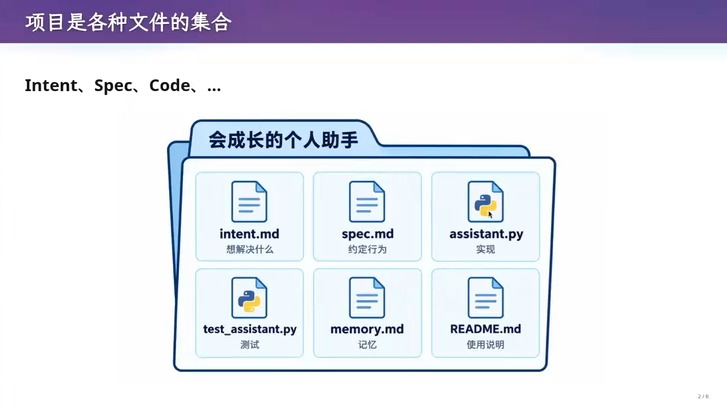
\includegraphics[width=\textwidth]{figures/fig_02_project_as_files.jpg}
\caption{项目是各种文件的集合：intent、spec、code、test、memory 各司其职\vtag}
\end{figure}
\srcnote{00:05:15--00:05:29}

\begin{lstlisting}[caption={幻灯片给出的“会成长的个人助手”项目文件布局与各文件职责}]
会成长的个人助手/
  intent.md          想解决什么
  spec.md            约定行为
  assistant.py       实现
  test_assistant.py  测试
  memory.md          记忆
  README.md          使用说明
\end{lstlisting}

幻灯片用 reminder.py 与 test\_reminder.py 演示：提醒时间从 10 分钟改成 30 分钟时，哪些实现和测试需要复查。为什么文件系统不够？1950 年、1960 年操作系统能给程序员的存储功能只有文件，关系型数据库尚未发明，程序员只能把项目存成文件；这是不断累积的历史将就。更根本的是，文件系统丢失了很多文件不适合表达的信息。讲者由此下判断：“我自己是觉得文件系统可能不是组织项目的正确的方式。”

\begin{figure}[H]
\centering
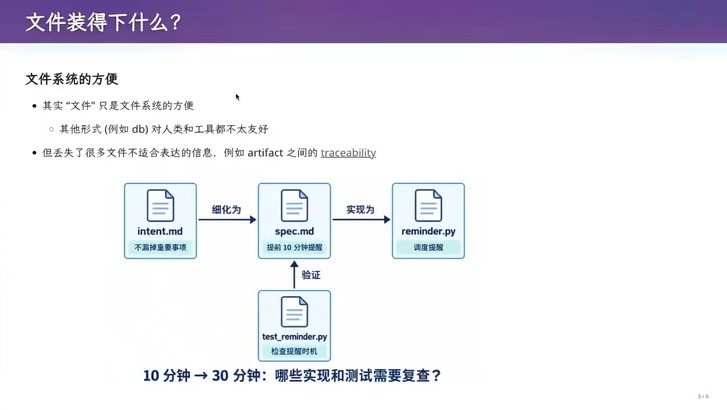
\includegraphics[width=\textwidth]{figures/fig_03_filesystem_convenience.jpg}
\caption{文件系统只保证“能存”，artifact 之间的 traceability 会丢失\vtag}
\end{figure}
\srcnote{00:06:45--00:06:59}

文件能装下 intent、spec 这类一条文档，测试用例的输入输出，以及程序运行中不能被违反的断言；装不下的是关联。典型例子是文档随手写“数据用链表管理”，AI 为性能把实现换成更高效的树结构，文档、代码、测试之间的关联没有被强行联系上，这就是技术债（technical debt）。随着文档与代码向前推演，不一致只会越来越多、不会越来越少，软件成为维护泥潭：拿出一份代码时说不清文档对还是代码对，聊天历史已经消失，换一台电脑后 git repo 里可能只剩一些 change 日志。

\begin{knowledgebox}{traceability 与技术债}
文件系统保存内容，却保存不了“谁对应谁”的关系；关联没有强制约束，不一致会随时间累积。讲者把“能否在演进中维持这种关联”称为 traceability（可追踪性），并指出这是软件工程里研究了非常长时间的问题。
\end{knowledgebox}

讲者用一篇论文说明问题由来已久：2014 年的综述“Software traceability: trends and future directions”，作者为 Jane Cleland-Huang、Orlena C.Z. Gotel、Jane Huffman Hayes、Patrick Mäder 和 Andrea Zisman，发表于 FOSE 2014，Pages 55--69，https://doi.org/10.1145/2593882.2593891，Published: 31 May 2014。所谓追踪，就是测试用例、哪怕文档中的一行、代码之间的关联是什么，能否在系统演进过程中仍然维持。

\begin{table}[H]
\centering
\begin{tabular}{p{3.6cm}p{2.8cm}p{7.2cm}}
\toprule
信息 & 文件系统能否表达 & 说明 \\
\midrule
intent / spec 文档 & 能 & 本质上是一条文档 \\
测试用例的输入输出、运行约束 & 能 & 可写成测试文件或断言 \\
文档与实现、测试之间的关联 & 不能 & 没有强制联系；文档写“链表”、实现被改成“树”，就形成技术债 \\
\bottomrule
\end{tabular}
\caption{文件系统能装下的内容与装不下的关联}
\end{table}

\subsection{本章小结}
项目由 intent、spec、code、test、memory、README 等文件组成，README 只承载最初的 intent 与最关键设计。文件系统能装下文档、测试与断言，却装不下 artifact 之间的关联；关联缺失累积成技术债。traceability 研究的正是这种关联能否在演进中维持。

\section{从 Git 快照到 AI 时代的软件形态}

文件系统装不下关联，人类只能“将错就错”：基于文件的工具从压缩包发展到 SVN、Git。讲者复述路径：用文件系统管理代码最终受不了，于是打压缩包发布、发给合作者，维护不下去，所以有了 SVN、有了 Git；随即提问“那下一个是什么，大家有没有想过下一个是什么？”幻灯片推论：AI 时代“软件”的形态会发生根本变化。如果以后人不再写代码，软件不必再是 Git Repo 里 readme.md、hello.c、docs 下的一堆文档，而可以把内容切成许多 object 或 entity，让文档、实现、测试彼此关联成一个有 cycle 的 graph——这种结构文件系统表达不了，更适合存进数据库，转录把它叫 report.db，后文又作 repo.db。人无法用 Unix 世界的工具维护它，讲者的方案是训练带强化学习反馈的 AI 去理解。

\begin{figure}[H]
\centering

\includegraphics[width=\textwidth]{figures/fig_04_ai_era_software.jpg}
\caption{将错就错的软件形态：从压缩包到 SVN、Git，AI 时代还会再变\vtag}
\end{figure}
\srcnote{00:10:30--00:10:44}

Git 管理的是文件、目录、快照和快照之间的关系。幻灯片用 A 加 feat 得到 B、Merge A 与 B 得到 C 说明并行开发与冲突：不同人在快照上分别开发，自然带来冲突；merge 汇合历史，rebase 把修改依次重放到新的起点。讲者称之为 Git 的哲学——小步前进：修一个 bug、改一个文档都产生一个 commit，多人各自提交，再用 rebase、merge、fast forward 或普通 merge，创建可追踪的整个项目的修改历史。

\begin{figure}[H]
\centering
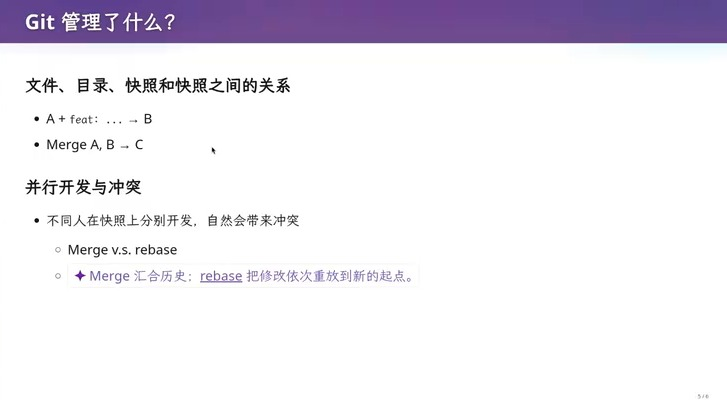
\includegraphics[width=0.92\textwidth]{figures/fig_05_git_manages.jpg}
\caption{Git 管理的是快照与快照之间的关系：merge 汇合历史、rebase 重放\vtag}
\end{figure}
\srcnote{00:13:30--00:13:44}

\begin{table}[H]
\centering
\begin{tabular}{p{2.2cm}p{5.6cm}p{6.4cm}}
\toprule
操作 & 对历史做什么 & 结果 \\
\midrule
merge & 汇合两条历史 & A 与 B 合并为 C，分叉被保留 \\
rebase & 把修改依次重放到新的起点 & 修改被重放，历史更接近一条直线 \\
\bottomrule
\end{tabular}
\caption{merge 与 rebase 的对比}
\end{table}

讲者设想由 AI 自动维护 artifact 之间的一致性：代码和文档必须一致（文档说链表，实现里必须是链表；文档说要 abc 三个方面的测试，test case 就必须有 abc）。任一大型系统里，只做一小步时绝大部分内容与这一步无关。于是 AI 可根据 chat 把相关文件和 test case 摘出来；AI 有动态生成任何内容的能力——everything is code、content is code，code 可以表达任何东西。讲者援引数据库概念（转录写作“VIO”，从上下文看指 view）：数据就在那里，却可以创建一个不一样的查询，以另一种形式展示。人看到的因此是一块可视化看板，列出与这次小步相关的内容，并反过来问“要改什么”；改完从 V0 到 V1，仍是同一个数据库。一次小步会把相关联的东西一起改：增加一种类型的测试用例，就在相关处补上测试、也可能改掉一些地方，从一个错综复杂关系构成的一致状态，到达下一个版本的一致状态。

演示中讲者打开自己的 report 仓库：有 assets、.cache 缓存系统、p1 到 p5、一些脚本；幻灯片的终端画面显示 assets、docs、guest、scripts 等目录，AGENTS.md、CLAUDE.md、Makefile、README.md 等文件，以及一长串以哈希结尾的 Markdown 笔记。

\begin{figure}[H]
\centering
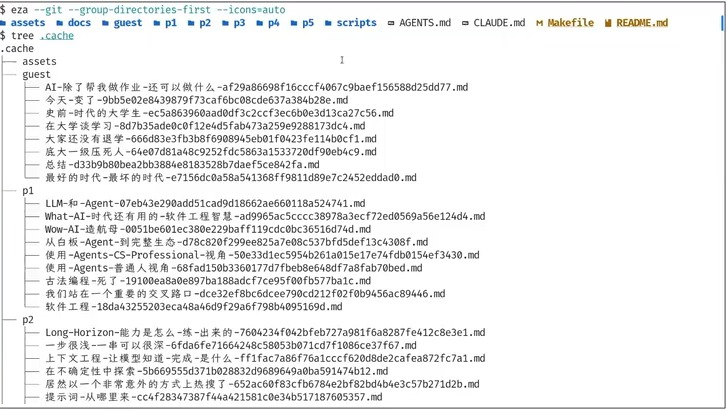
\includegraphics[width=\textwidth]{figures/fig_06_repo_tree.jpg}
\caption{一个真实仓库的目录：assets、docs、guest、scripts 与 AGENTS.md 等\vtag}
\end{figure}
\srcnote{00:15:15--00:15:29}

\begin{importantbox}{一次小步对应一个视图}
大型系统里任意一次小步只牵动少量 artifact。让 AI 依据这次对话把相关文件、测试和文档摘出来，动态生成一块看板；改动只发生在这张相关子图上，改完仍落回同一个仓库数据库。
\end{importantbox}

讲者把这种变化称为软件工程“就又变了，彻底变了”，并给出判断与限定——“我觉得这是一个未来有可能发生的，就是在 AI 内部，它是这样生产软件，然后从此以后我们也就再也不要看代码了”。对照之下，cursor 等现代 IDE 打开后默认进入 agent mode，原来熟悉的 IDE 没有了，人被推着用聊天的方式沟通；讲者说自己相对来说比较精通“古法编程”，对代码仍有一些掌控欲，并补了一句“可能是不好的”。

\subsection{本章小结}
文件工具从压缩包走到 SVN、Git；Git 管理文件、目录、快照及其关系，merge 汇合历史，rebase 重放修改，都服务于小步前进。当 Agent 成为主要生产者，讲者设想把 artifact 关系图存进数据库（report.db / repo.db），由 AI 维护代码、文档与测试的一致性，人只面对针对当前小步生成的看板。这个方向被他限定为“未来有可能发生”。

\section{AI 时代的软件工程智慧与「学生思维」}

讲者回答「模型强到能一步生成整个项目，学软件工程还有没有用」时，把握有限。他连用四个限定词，「可能是不好的」「这可能是不对的」「但是就未来可能会是」「这可能是一个途径」，随后说「这个怎么做，我们现在还不知道」。即便发生，构造新东西借用的仍是计算机科学的经典概念：数据库的视图、实体和关系，以及 Git 的模型。「就这个模型没有变」——Git 长期开发经验要求「一步一步向前」，在「一步生成」底下「我们是大步向前的，那就惨了」，所以至少在初期「我们可能还是要沿用过去的，大家积累的软件工程智慧去小步向前」。目标叫「通往极乐的世界」，语气是「我还是相信……有可能」。

\begin{importantbox}{三种断言强度}
三类陈述必须分开：讲者的预测与愿望（「我相信」「有可能」）、转述的既有经验（Git 主张小步前进）、明确承认的未知（一步生成「我们现在还不知道」）。不要把未知当作论据，也不要把「极乐世界」写成已发生的事实。
\end{importantbox}

\subsection{为什么学生遇不到 rebase}

上节课讲者问「什么是 Git Rebase」，大多同学答不上来；一位已毕业的同学解释，学生时代大多数人不会合作，做作业基本单分支开发，rebase 与 merge 用武之地很少，他给 git rebase 打了 0/10。讲者先承认「正确，这个 point 是对的」「你们做作业的时候确实不会」，再反驳由此推出的不学：你真去外面走一走，「这个互联网开发者社区铺天盖地都是」合作，总会留意别人的项目、看到 CONTRIBUTING.md。他当场让 Agent 在 \texttt{/home/jyy/Projects/GenSE} 里演示搜索贡献者指南。

\begin{lstlisting}[language=bash, caption={在 GenSE 仓库中搜索贡献者指南并查看仓库约定（依视频终端画面整理）}]
$ cd /home/jyy/Projects/GenSE
$ find . -iname "*CONTRIBUT*" 2>/dev/null | head -20; echo "---"; ls docs
slice-format.md
Sway-cheatsheet.html
$ head -40 README.md; echo "==git=="; git log --oneline -5 2>/dev/null
465561d Refresh p4 AI caches
e3e0a46 Rework p4 Lect ...
ea51872 Rework p4 Lect agent-era VCS sections (worktree workaround, MVCC vs locks, no-blame)
\end{lstlisting}

结果一个都没有。Agent 于是先列出这份指南通常应覆盖什么，再与仓库现有的分散约定对照——约定不是不存在，只是散落在别处。

\begin{figure}[H]
\centering
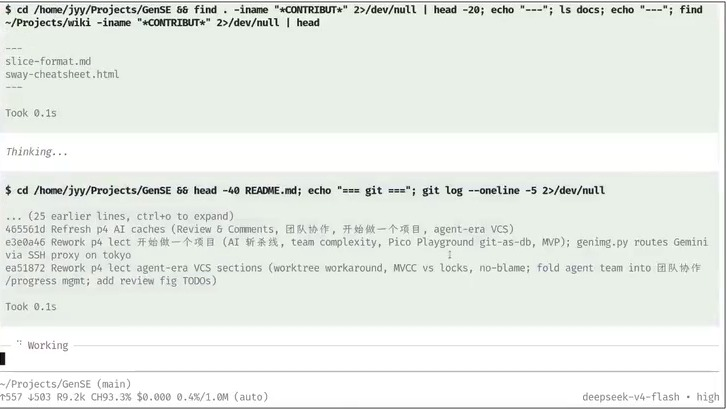
\includegraphics[width=\textwidth]{figures/fig_07_search_contributing.jpg}
\caption{让 Agent 先在仓库里搜索 CONTRIBUTING.md，结果为空，于是转向定义这份指南应该写什么\vtag}
\end{figure}
\srcnote{00:20:15--00:20:29}

\begin{figure}[H]
\centering
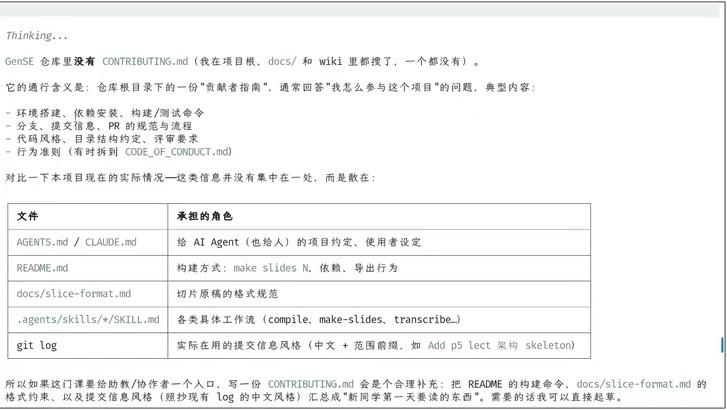
\includegraphics[width=\textwidth]{figures/fig_08_contributing_checklist.jpg}
\caption{贡献者指南的应有清单，以及它在 GenSE 仓库中对应的分散文件\vtag}
\end{figure}
\srcnote{00:20:30--00:20:44}

\begin{knowledgebox}{CONTRIBUTING.md 应该写清楚的约定}
Agent 的清单：环境搭建、依赖安装、构建与测试命令；分支、提交信息、PR 规范与流程；代码风格、目录约定、评审要求；行为准则（可拆到 \texttt{CODE\_OF\_CONDUCT.md}）。GenSE 仓库把同类信息分散在 \texttt{AGENTS.md} / \texttt{CLAUDE.md}、\texttt{README.md}、\texttt{docs/slice-format.md}、\texttt{.agents/skills/*/SKILL.md} 与 git log 的提交风格里，建议汇总成「新同学第一天要读的东西」。
\end{knowledgebox}

\subsection{从「学生思维」到 AI 时代的斩杀线}

讲者称「其实不是批评大家」：高中的规则是老师不教的就是你不需要会的、考试不考的就是你不用学的，这在升学利益最大化下正确，带进大学就成了「新人类和旧人类之间的 gap」。对策是在操作系统、编译器、软件工程等经典课上形成自己的理解（first principles）。

危机是 AI 时代「斩杀线以下的价值就全部归零」。线画在哪里，他判断「可能还展不到各位 985……计算机专业的同学」；低级智力劳动不同——会计从业者「好像我看过一个报道说，中国可能是不是有一千万，还是有多少」，行业顶端暂时没有威胁，底下大量人面临被 agent 替代。「一千万」是带疑问转述的报道数字，原样保留，不作统计结论。

\begin{importantbox}{本节的因果链}
模型或许在「一两年以后」能一步完成大型项目（不确定）——即使发生，新范式仍复用经典概念——经典课程的价值不会被抹平；反过来，「老师不教就不必学」会主动放弃这种价值。
\end{importantbox}

\subsection{本章小结}

本节处理的是技术判断的边界：用「可能」「我相信」「我们现在还不知道」限制对未来的推断，用开源社区的现实反驳「用不到 rebase 所以不必学」；经典课程里的智慧仍是构造新事物的材料。

\section{Git 管理什么：快照、merge 与 rebase 的取舍}

\subsection{快照与两个开发者}

Git 管理的是快照，即一个目录在某一时刻的样子，以及快照之间的关系；两个开发者 A、B 在各自的快照上独立小步开发，承载对象是 commit。

\subsection{merge 的作者归属问题}

Git 的原始模型「相对来说是不那么提倡使用 rebase 的」，它主张两路 merge：新提交有两个 parent，继承两条线上的修改。代价在归属：merge 由 A 执行时，B 写的内容「它做的就变成 A 了」，是「隐藏的作者修改」；B 单独加的一行「可能还能追溯到 B」，但冲突在 resolve 之后完成时，「这个 change 就是由 A 完成的」「B 改的代码，最后 ownership 又归到了 A」。讲者称这是「相对来说有一点小小的小麻烦」，它正是 rebase 存在的理由。

rebase 不制造汇合的提交，而把一条线上的修改依次重放到另一条线的后面：A 先改文档、加测试，B 加 feature、加测试，rebase 把 feature 放到 A 之后，再把测试放过来。边界有两处：feature 与已有测试用例不兼容，或两人改了同一处、做出「两个完全不兼容的东西」，重放就进行不下去；只有「完全没有任何冲突」，才能一路合过去变成线性历史。

\begin{warningbox}{rebase 的失败边界与代价}
一旦冲突就要 resolve、进入 rebase 模式；搬 feature 可能失败，搬 test 可能再次失败，每次都创建新提交。commit 带 ID：两路 merge 保留所有原 ID 并新建一个，而 rebase 因改掉快照的 base，每次都会创建新的 commit ID，历史随之改变。学生进入这个模式会「瞬间自己就不知道应该怎么办了」，然后打开 agent。
\end{warningbox}

\subsection{我们真正想操作的是 change}

概念诊断：真正想操作的是 change（一次修改），但 Git 没有专门的 change 对象，用 commit 连同 commit 与 parent 的关系充当一次修改，于是有「一点点轻微的不一致」——你希望「把这个修改搬过来」，搬动的却是会变 ID 的提交。推论：把 change 变成 first-class citizen（一等公民），就得到「下一代更好用的版本控制系统」。

\begin{figure}[H]
\centering
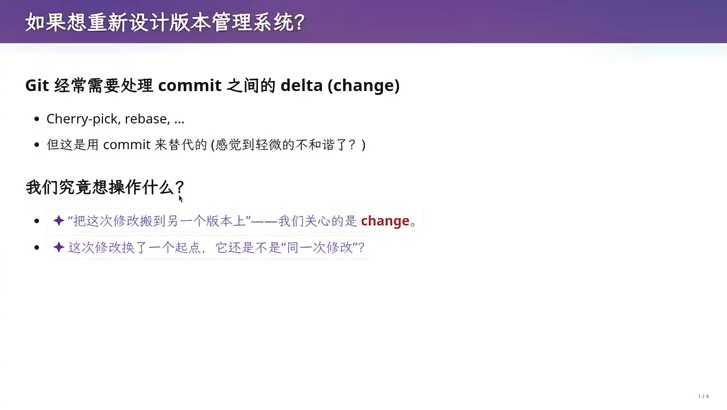
\includegraphics[width=\textwidth]{figures/fig_09_redesign_vcs.jpg}
\caption{Git 经常需要处理 commit 之间的 delta（change），cherry-pick、rebase 都属此类；问题在于它用 commit 替代了 change\vtag}
\end{figure}
\srcnote{00:22:45--00:22:59}

\subsection{本章小结}

Git 的数据模型是快照加父子关系，合并默认走两路 merge，代价是把 B 的修改在提交层面记到 A 名下；rebase 用重放换回线性历史，代价是可能反复失败并产生新 commit ID。更底层的问题是工具缺少 change 抽象。

\section{把 change 作为一等公民：Jujutsu 的设计推论}

\subsection{change ID 与 commit ID}

用一个前提——「change 是一等公民」——讲者推导出 Jujutsu（命令名 jj）的设计：它与 Git 底层完全兼容，可直接当 git 用，增加的正是 change 概念，每个提交可 assign 一个 change，rebase 时把 change 搬过去。幻灯片写「祝贺，你发明了 Jujutsu——a version control system」，主张「Rebase 不应该让同一次 change 失去身份」。解法是把标识分开：commit ID 会变，change ID 延续，同一次修改可有不同修订版本。Git 视角下重写历史只得到一组新 commit，不显式记录新提交是旧提交的下一版；jj 视角下提交变了而 change 身份延续，能明确知道新旧提交分别是谁的后续修订版。

\begin{figure}[H]
\centering
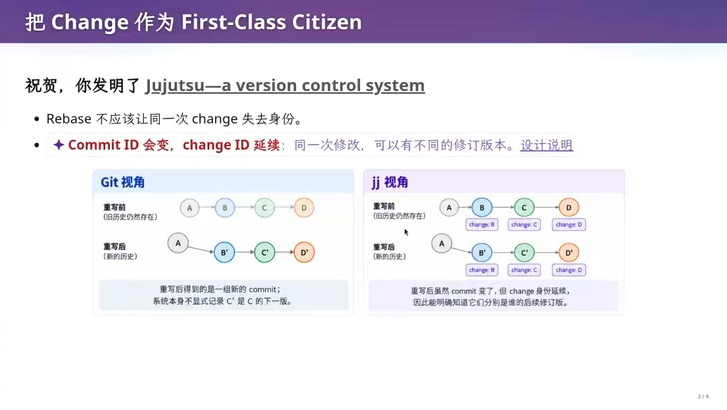
\includegraphics[width=\textwidth]{figures/fig_10_change_first_class.jpg}
\caption{把 change 作为一等公民：Git 与 jj 在历史重写后的身份记录方式对照\vtag}
\end{figure}
\srcnote{00:28:45--00:28:59}

\begin{tabular}{p{5.5cm}p{8.5cm}}
\toprule
Git 视角 & Jujutsu（jj）视角 \\
\midrule
重写历史后得到一组全新的 commit & 重写历史后 commit 也变了，但 change 的身份延续 \\
系统不显式记录 C' 是 C 的下一版 & 能明确知道新旧提交分别是谁的后续修订版本 \\
commit ID 会变 & change ID 延续，同一次修改可以有多个修订版本 \\
\bottomrule
\end{tabular}

冲突本身仍解决不了：「在 rebase 时遇到冲突，这是解决不了的」；但有 change 对象后可把 change 一路带下来、直接 rebase 到目标，中间引入许多冲突，再由系统自己的一套记录塞进去，之后统一 resolve。评价是「底层的模型没有变，但是你用起来会舒服很多」。

\subsection{未完成的工作也有位置}

jj 不需要 staging area——暂存区，Git 中工作区与提交之间的缓冲。工作副本本身就是一个 commit：多数 jj 命令自动记录文件修改并更新它，像「一直在 commit+amend」；改一个字节就立即提交，并「先把上一次的 commit 给抹掉」，用当前修改替代，仓库永远处于已提交的 change 状态。

\begin{lstlisting}[language=bash, caption={讲者口述的 Git 痛点流程：把改到一半的工作放进 index 再 stash}]
$ git add hello.c
$ git stash
\end{lstlisting}

中断场景说明其价值：hello.c 改到一半，不能编译、不能运行、测试不通，偏巧要一分钟内修更高优先级的 bug；不应 commit，正确动作是加进 index 再 git stash。中断还会叠加：刚修一半又被更高优先级 bug 打断，只能再 stash，stash 堆了许多提交还要管理。结论：你无时无刻不在编辑这个仓库，「这不就是一个 change 吗」，给 hello.c 加一行、减一行，都是 change。

最激进一步是冲突处理：幻灯片把「冲突直接存进 commit」标为 killer feature——Rebase 可直接完成、之后统一处理；保存的是冲突的逻辑表示，带着冲突的 commit 仍能继续 rebase、merge。设计启发是把「尚未解决」表达成可保存、可继续操作的状态。

\begin{figure}[H]
\centering
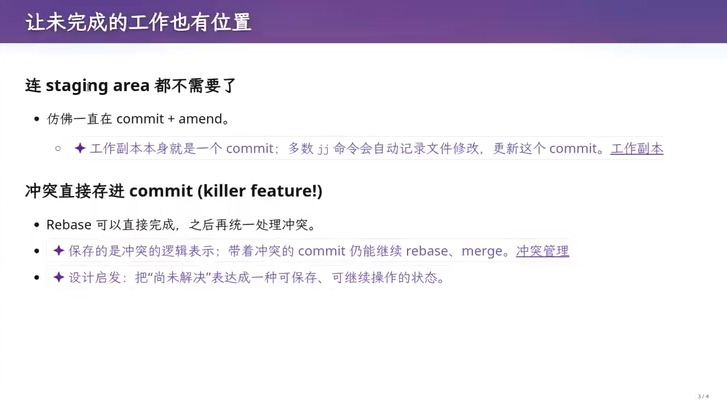
\includegraphics[width=\textwidth]{figures/fig_11_work_in_progress_commit.jpg}
\caption{工作副本本身就是一个 commit，未完成的工作因此有位置；冲突直接存进 commit\vtag}
\end{figure}
\srcnote{00:30:00--00:30:14}

\begin{knowledgebox}{从一个前提推出的三个设计}
把 change 提升为一等公民，视频依次得到三件事：change 有独立身份，rebasing 后 change ID 延续而 commit ID 重写；不需要 staging area，工作副本本身即 commit，编辑即更新提交；冲突可被保存，带冲突的提交仍能继续 rebase 与 merge，解决冲突从「必须先解决才能继续」变成「可以稍后统一处理」。讲者声明「这不是它的全部」。
\end{knowledgebox}

\subsection{肌肉记忆与学习顺序}

讲者已形成 Git 肌肉记忆，比他更老的一代是 SVN 肌肉记忆，一旦形成「要把这个习惯掰过来，就很困难了」。他自陈即便理解 jj、能从 first principle 出发、相当于「virtually re-implement 这个系统」，也「没有足够的时间再去训练另外一个肌肉记忆」。学生反过来：还没形成记忆时直接用对的东西，先记住最正确的设计，再理解，再回望历史。

历史是积累的：SVN 用不下去了才有 Git，Git 被发现有缺点之后有了 jj。Git 出现时因是 persistent data structure 显得先进，而 SVN「从一开始，它从 Diff 那条线就走错了」；现在回看 Git 也犯了一些设计上的问题——最早没想过 rebase 有这么大的 impact，有 merge 已能解决手上问题，所以「可能没有把这个概念模型想的更加更加的清楚」。幻灯片用 Einstellung effect 解释锁定：熟悉的解法占住注意力，棋手说在寻找更优解，目光却仍围绕旧套路（2008 年眼动实验）。换代机会来自尚未形成肌肉记忆的人。

\begin{figure}[H]
\centering
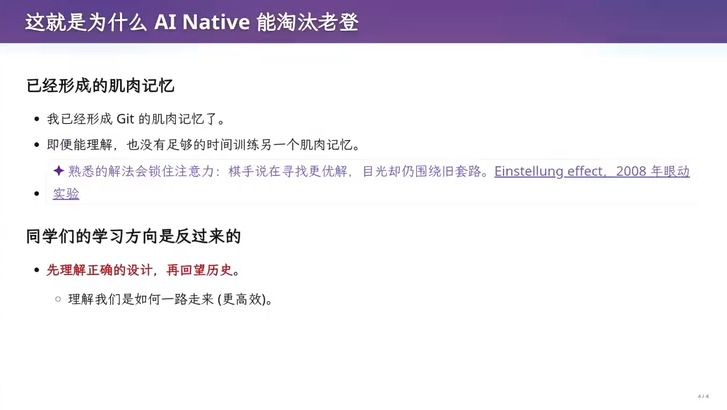
\includegraphics[width=\textwidth]{figures/fig_12_einstellung.jpg}
\caption{Einstellung effect：已经形成的肌肉记忆锁住注意力，学习方向应当反过来\vtag}
\end{figure}
\srcnote{00:33:45--00:33:59}

讲者以自我定位收束：「但这门课不是软件工程，这门课是生成式软件工程。」下一张幻灯片的标题是「Agent 时代，再次重新设计版本管理系统」，其要检查的隐含假设是使用者为人类。

\begin{figure}[H]
\centering
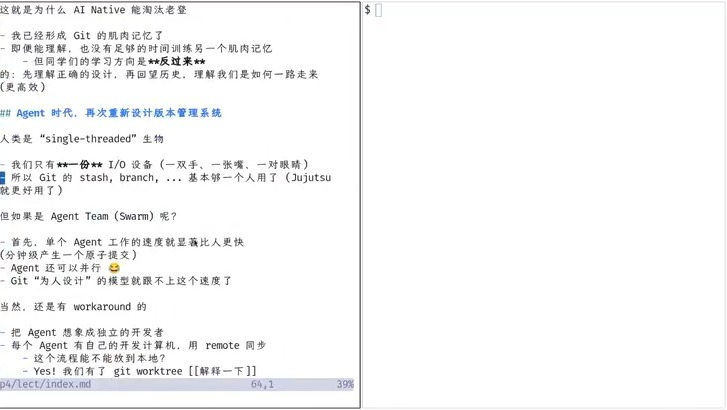
\includegraphics[width=\textwidth]{figures/fig_13_agent_redesign_title.jpg}
\caption{章首：Agent 时代，再次重新设计版本管理系统\vtag}
\end{figure}
\srcnote{00:35:45--00:35:59}

\subsection{本章小结}

Jujutsu 两个卖点来自同一抽象：change 被系统命名后，身份能在历史重写中延续，未完成工作也通过「工作副本即 commit」获得位置。讲者认为它对人类更友好、可能对 agent 也稍友好，但承认自己受限于肌肉记忆无法切换。可迁移的是那条推导：先确定真正想操作的对象，再让工具的数据模型围绕它设计。

\section{当版本管理系统的使用者不再是人}

\subsection*{本节回答的问题}
Git 已是分布式版本控制的成熟答案，为什么到了 agent 时代还要重新设计它？

\subsection{一个被所有工具默认的前提}
讲者把落点讲得很直接：要在 agent 时代再次重新设计版本管理系统。他不否认让 agent 直接用 Git 可行，也承认 agent 好像很会 rebase；但他判断 Git 对人类的进步远大于对 agent，因为从 SVN 到 Git，所有 version control system 都默认使用者是人类。字幕里的 get 指 Git，Dipsick V4 Flash 指画面中的 deepseek-v4-flash。

\subsection{人是单线程生物}
视频用操作系统课的类比解释人的限制：线程像一个人，访问共享内存只有 load 和 store（read 和 write）两个基本操作，读写不能同时发生，要同时就得诉诸原子指令。讲者把“人”放回模型：观察世界时手背在身后只能看，要写变量必须闭眼；闭眼期间寄存器里的值已经过期——中间可能被换下 CPU、被中断，换成另一个线程执行一秒，于是他闭眼扔出的粉笔导弹很可能打错位置。人的 I/O 只有一份：一双手、一张嘴、一对眼睛；人与人之间存在无法逾越的物理屏障，谁也进不到对方的思想里。

\begin{figure}[H]
\centering
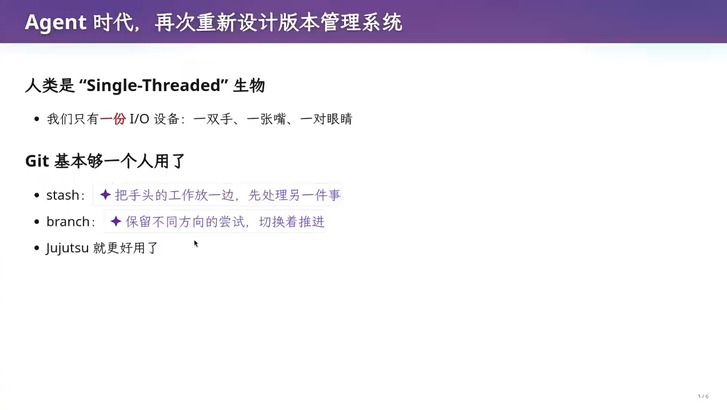
\includegraphics[width=\textwidth]{figures/fig_14_single_threaded.jpg}
\caption{人是 single-threaded 生物：只有一份 I/O 设备，stash、branch 一类机制都是为单个开发者设计的\vtag}
\end{figure}
\srcnote{00:36:00--00:36:14}

\begin{importantbox}{整场讲座的公理}
所有既有版本控制系统都假设使用者是人类。人的 I/O 只有一份，状态无法直接共享；由此推出的并发模型（单线程、读改写非原子、需要原子指令）恰好就是人做修改时的模型。讲者据此反问：agent 时代的局限与要打破的改进分别是什么。
\end{importantbox}

\subsection{时间尺度：为什么 stash 与 branch 曾经够用}
换算成工程时间：人产生一次 change 以小时为单位，一个模块十几个人已是不小的团队，团队最多以十分钟为单位产生一次提交；而工位旁的确认只要 20--30 秒，公司里 leader 每天早会用半小时划分 scope。沟通比提交快，所以“把工作放一边”的 stash 合理——导师在你改到一半时再打电话的概率很低，stash 通常只有一层，层多了要 rebase，人也可以拒绝低优先级工作、自己排队。

\begin{center}
\small
\begin{tabular}{p{2.2cm}p{5.6cm}p{5.6cm}}
\toprule
维度 & 人类开发者（古法编程） & 单个 Agent \\
\midrule
产生 change 的量级 & 小时级；十几人团队约十分钟一次提交 & 分钟级，甚至更快 \\
一次修正的耗时 & 一两个小时 & 上下文热时几十秒；模型几秒钟 \\
可扩展规模 & 一个模块十几个人已是不小的团队 & 可轻易得到 10 倍、100 倍的 agent team \\
同步方式 & 工位旁 20--30 秒确认、每天早会分派任务 & 主 agent 协调、观看输出、inject prompt \\
\bottomrule
\end{tabular}
\end{center}

\subsection{本章小结}
Git 精确服务了一个单线程、I/O 有限、彼此无法直接共享状态的使用者；使用者换成 agent，前提失效，重新设计才有理由。

\section{Agent Team 的速度与 worktree 的本地并行}

\subsection*{本节回答的问题}
当执行者从一个 agent 变成一支 agent team，为什么面向人设计的 Git 会跟不上？把“每个 agent 一台机器”的远程模型搬到本地需要什么机制？

\subsection{从分钟级到秒级的原子提交}
讲者划出分水岭：Git 是给人用的，但在 agent 时代这件事变了。单个 agent 生产 AI slop 以分钟级为单位、甚至更快，上下文热时修一个东西只要几十秒，deepseek-v4-flash 几秒钟就能完成；当 agent 能秒级产生原子提交，又能轻易扩展出 10 倍、100 倍的 team 时，按人类时间尺度设计的版本管理模型就有点跟不上。反向证据是门控：大型项目的测试流水线本身要跑几分钟，会放缓提交，但 agent 毫无疑问加速了开发；需要加速的不只是产生提交，还有协调、验证与整合。

\begin{figure}[H]
\centering
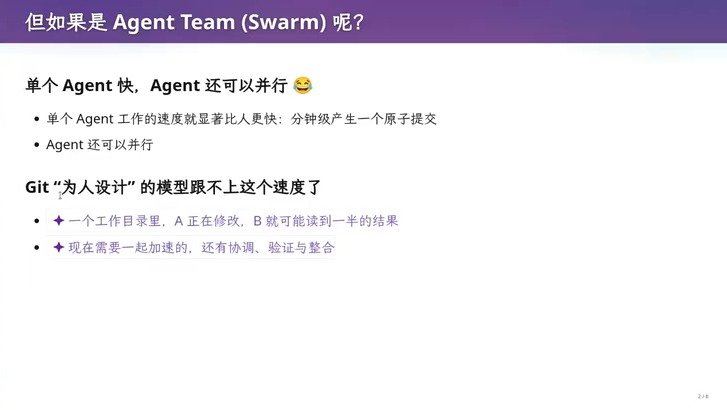
\includegraphics[width=\textwidth]{figures/fig_15_agent_team_swarm.jpg}
\caption{Agent Team（Swarm）：单个 agent 快、还能并行，分钟级原子提交与并行写入让为人设计的 Git 模型跟不上\vtag}
\end{figure}
\srcnote{00:41:00--00:41:14}

\subsection{把每个 Agent 当成独立开发者}
最省事的方案是让每个 agent 有自己的开发计算机（可能是容器），用 remote 同步，把单线程的人与 agent 一一对应。讲者的指令模板：我的 remote 仓库在 Git，你现在是单人开发者，可以从 tmux 收到命令。演示里两个 tmux session 放在两台不同机器或容器上，物理隔离、互相看不到；命名用了 master 与 slave，讲者自嘲这是“还故意用一个可能在中国现在还能用的词”。本地化版本是幻灯片给出的 git worktree：一个仓库、多个工作目录，每个 worktree 有自己的工作文件、HEAD 和 index（暂存区），共享对象库与分支引用，提交本地直接可见，无需互相 push 或 pull。

\begin{figure}[H]
\centering
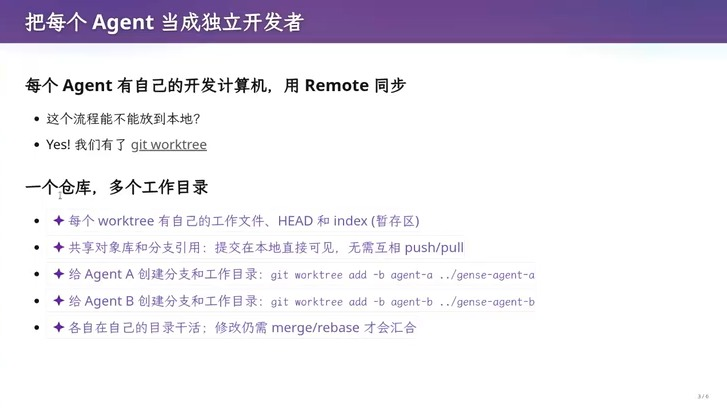
\includegraphics[width=\textwidth]{figures/fig_16_git_worktree.jpg}
\caption{git worktree：一个仓库、多个工作目录，每个 worktree 各有 HEAD 和 index，共享对象库与分支引用\vtag}
\end{figure}
\srcnote{00:42:15--00:42:29}

\begin{lstlisting}[language=bash, caption={把远程协作搬到本地：幻灯片给出的 worktree 命令，以及演示中工头调度两个会话的命令（与画面逐字一致）}]
# 幻灯片给出的两条命令
$ git worktree add -b agent-a ../gense-agent-a
$ git worktree add -b agent-b ../gense-agent-b

# 演示中让两个 tmux 会话进入各自 worktree 并启动 pi
$ tmux send-keys -t slave-a 'cd /tmp/fancy-worktrees/slave-a; pi' C-m
$ tmux send-keys -t slave-b 'cd /tmp/fancy-worktrees/slave-b; pi' C-m
$ sleep 10
# 用 capture-pane 读取会话、用 grep working 判断忙闲，空闲才发键
$ tmux capture-pane -p -t slave-a -S -20 | tail -25
# 用 pgrep 与 /proc 定位每个 pi 进程真实的工作目录
$ for p in $(pgrep -x pi); do echo "pid=$p cwd=$(readlink /proc/$p/cwd)"; done
\end{lstlisting}

\subsection{现场演示与失败边界}
演示环境：\texttt{fancy-project} 仓库（git version 2.47.3）、fish、编码 agent \texttt{pi}（v0.85.1，模型 deepseek-v4-flash）；两个 tmux 会话重命名为 slave-a 与 slave-b，被送进 \texttt{/tmp/fancy-worktrees/slave-a} 与 slave-b 两个 worktree。讲者称调度为“工头”：用 tmux send-keys 把指令打给对方 pi，靠 capture-pane 与 grep working 判断忙闲，空闲才发键，避免指令糊进正在生成的输入框。任务是各写一坨超过 1000 行的 slop；生成器固定 seed=2026、用模板拼函数名，产物可复现，一处已到 1179 行，\texttt{slop\_a.py} 快照为 5234 行、约 177KB、含 240 个 \texttt{verb\_noun\_XXXX} 样板函数，\texttt{self\_test()} 的 29 项全部通过、CLI 各子命令可运行。这些代码内容低信号：重复的 acc += (idx * i) \% 97、scratch.append(...)、千篇一律的 docstring 与 try/except。多 agent 形态是一个监工 agent 协调子 agent：由 Codex 设计、Claude review，让它们互相打架再达成一致，主 agent 只观看输出、总结并注入 prompt。

\begin{figure}[H]
\centering
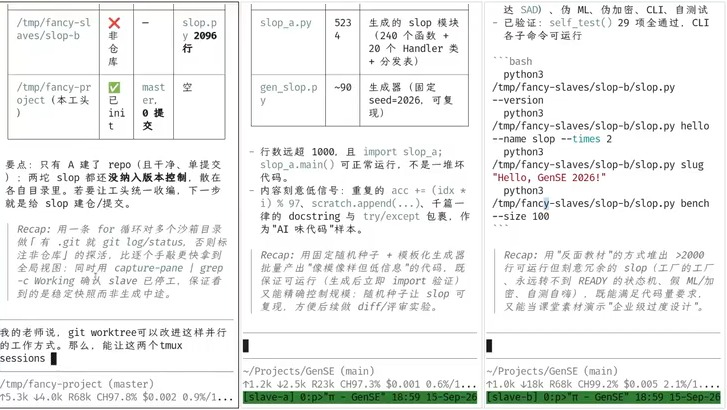
\includegraphics[width=\textwidth]{figures/fig_17_worktree_demo.jpg}
\caption{两个 worktree 并行生成 slop 模块：调度表里 slave-a 先建仓库、slave-b 写代码，产物 5234 行、self\_test 29 项通过\vtag}
\end{figure}
\srcnote{00:45:30--00:45:44}

讲者对比仓库状态后指出：工作在同一 Git 仓库上会有麻烦，在不同 repo 上就完全可以——可以拉别人的提交、冲突自己修，必要时给 master agent 发消息。worktree 正是这条边界的 workaround。他还给了一条方法论：提问是关键，看到 git worktree 或某个 sandbox container 就可以立刻让 agent 试一试。

\begin{warningbox}{worktree 不是合并方案}
worktree 提供的是更轻量的本地协作与空间隔离。讲者的限定很清楚：有冲突的修改仍然需要 merge 与 rebase 才能合并。它解决工作目录互相踩踏，不解决修改语义上的冲突。
\end{warningbox}

\subsection{本章小结}
Agent 把提交速率推到分钟级乃至秒级、并行度推到 10 倍、100 倍，而 Git 的尺度仍按人类设定。让每个 agent 独立开发、用 remote 同步是第一种答案，git worktree 给出了更轻的本地版本。

\section{worktree 的机制与版本控制的第一性需求}

\subsection*{本节回答的问题}
worktree 凭什么能在同一台机器上制造隔离？版本控制真正要解决的问题来自哪里？

\subsection{一个仓库，多个工作目录}
worktree 的心智模型是：Git 允许创建一个工作树，可以把它想象成连接到一个 remote、一个 Git repo，在里面做独立提交。关键是 \texttt{.git} 的两种形态：常规仓库里 \texttt{.git} 是目录，含 logs、objects 和“三种类型的对象”；worktree 里 \texttt{.git} 是普通文本文件，内容写着 gitdir，指向主仓库下的一个目录。这体现 Git 极大程度复用了操作系统的机制：worktree 目录是一个小型 Git 目录，仍有 HEAD、index、logs，却依附原有 \texttt{.git} 目录而生。提交在本地直接可见，不需要互相 pull 和 push，比开好几台虚拟机各放一个 agent 更轻量。

\begin{figure}[H]
\centering
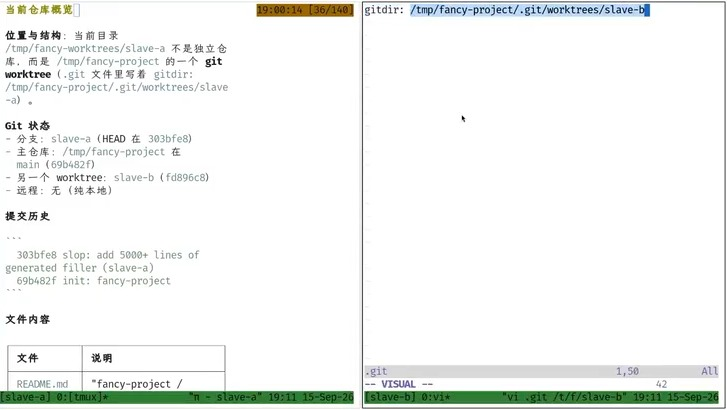
\includegraphics[width=\textwidth]{figures/fig_18_repo_overview_gitdir.jpg}
\caption{worktree 的 .git 是一个 ASCII 文本文件，里面写着 gitdir 指针，指向主仓库的 .git/worktrees 目录\vtag}
\end{figure}
\srcnote{00:49:30--00:49:44}

\begin{lstlisting}[language=bash, caption={worktree 的 .git 是文本文件而非目录：识别命令与目录内容（与终端画面一致）}]
$ file .git
.git: ASCII text
$ vi .git
gitdir: /tmp/fancy-project/.git/worktrees/slave-b
$ cd /tmp/fancy-project/.git/worktrees/
$ tree slave-b/
slave-b/
  COMMIT_EDITMSG
  commondir
  gitdir
  HEAD
  index
  logs
  ORIG_HEAD
  refs
3 directories, 7 files
\end{lstlisting}

仓库状态可逐项核对：worktree slave-a 不是独立仓库，分支 slave-a 的 HEAD 在 303bfe8；主仓库 \texttt{/tmp/fancy-project} 在 main 上，提交 69b482f；另一个 worktree slave-b 位于 fd896c8；远程为空。提交历史两条为 slop: add 5000+ lines of generated filler (slave-a) 与 init: fancy-project。

\subsection{回到为什么需要版本控制}
讲者拉回第一性：为什么需要版本管理。回答是人的限制塑造了工具——人的生产效率有限，人之间有 communication gap，沟通效率极低，就算沟通也可能出错；正因为这个缺口，团队每天早上才要开会同步进展、分派任务。他用室友请教数学题量化成本：明明你会做，却怎么都讲不明白，除非你是好老师、能共情别人。沟通成本决定了团队能长到多大：系统变大、人变多，沟通效率降低，产出速度下降，100 人的团队不可能达到 10 人团队效率的 10 倍，能有两三倍已经不错。

\begin{figure}[H]
\centering
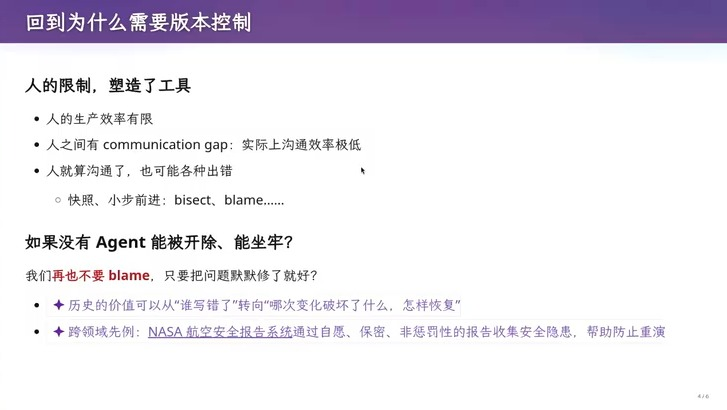
\includegraphics[width=\textwidth]{figures/fig_19_why_version_control.jpg}
\caption{人的限制塑造了工具：生产效率有限、沟通效率极低且会出错，于是需要快照、小步前进、bisect 与 blame\vtag}
\end{figure}
\srcnote{00:51:15--00:51:29}

\begin{knowledgebox}{本段没有展开的部分}
幻灯片上还有更远的推论：如果没有 agent 能被开除、能坐牢，是否还要 blame，历史的价值会不会从“谁写错了”转向“哪次变化破坏了什么、怎样恢复”，并援引 NASA 航空安全报告系统的自愿、保密、非惩罚性报告机制。讲者在本片段只讲到“人的限制塑造工具”与沟通成本，blame 与 NASA 出现在 00:52:00 之后，不应提前归入本段结论。
\end{knowledgebox}

\subsection{本章小结}
worktree 靠一个 gitdir 文本文件把隔离与共享同时做到，却没有改变冲突需要合并。版本控制的根本动力始终是人的局限：生产效率有限、沟通成本高、彼此状态不可见。

\section{工具为何长成现在的样子：人的限制与 blame 的消亡}

版本管理工具的形态由人的限制塑造，这是讲者理解 Git best practice 的起点。人生产效率有限，彼此之间存在 communication gap，就算沟通了也可能出错：室友向你请教一道数学题，你明明会做却讲不明白，除非你是很好的老师、能共情并站在别人角度思考。沟通成本既然如此之高，团队才需要每天早会同步进展、再分派任务。规模收益也随之递减——一个 100 人的团队不可能达到一个 10 人团队效率的 10 倍，“可能有两倍三倍就已经挺不错了”。团队无法无限变大，于是有了快照与小步前进：改一个 typo 也做一次 commit，每个小 commit 都可追溯。

追溯真正依赖的是人。回溯到某人某次提交的时刻，他还能想起当天早会、收到的需求与沟通出的问题，甚至找到当时的沟通记录文档；bisect 与 blame 正是为这种“有记忆、可追问的人”设计的。

\begin{knowledgebox}{小步提交为什么有效}
快照只是数据，让它变成经验的是人对时间点的记忆。bisect 与 blame 把问题定位到“某个人做某件事的那一刻”，而那个人恰好能补上缺失的上下文。
\end{knowledgebox}

若执行者换成 agent team 或 agent swarm，blame 的前提就消失了：人可以 blame，因为被 blame 者会承担后果——“我 blame 你多了，你就该被开掉了，实习生你就背锅了”；agent 没有坐牢、被开除的能力，“我们再也不需要 Blame 了，我们的项目只要前进就可以了”。何况现在的每个 agent 都是相同的模型，是完全相同的克隆体；同一件事交给它们，虽然模型有不确定性、可能有细微差别，但方向性的结果大概率收敛。于是历史的价值从“谁写错了”变成“我怎么把它修好”：不必追查哪个提交引入错误，只要把错误修掉。快照仍必须保留——方向走错后，没有历史的某个 snapshot，走远了再回头的代价更大；但姿态是“大步向前”，“几乎永远不要看过去”，commit 里留下一些 lessons 和项目的演化轨迹。

\subsection{本章小结}

人的限制塑造工具：高沟通成本与次线性的团队收益催生快照、小步提交，bisect、blame 服务于可问责的人。执行者变成同构、不可开除的 Agent 后，blame 前提消失，历史从追责转向支撑修复与继续前进。

\section{把版本管理当作并发控制：从乐观假设到悲观上锁}

讲者用并发控制的框架理解 Git 与 Agent 协作，措辞是“有点像”“像是”，因此这是类比，不是 Git 的官方定义。数据库里，两条 SQL 各自是一个很大的 transaction，中间可混任何代码：先 select 读，再执行图灵完备的计算（python 或 JavaScript，甚至读取当前时间），最后 update。两个事务交叉读写就会冲突；update 互相要读对方、或我要锁你的对象而你要锁我的对象，就形成循环依赖即死锁，事务只能 abort、回滚重来。

Git 属于乐观一侧：先假设两个 transaction 不冲突，让双方各自往前跑，到合并（merge 或 rebase）时再检测，并相信“大概率不会产生冲突”。该假设靠访问局部性成立——学生选课读写的都是自己那块数据，两人同时选课也互不干扰；软件工程里则是事前开过会（“今天早上开过会了”），各人分头做，合并大概率顺利。

\begin{importantbox}{乐观并发控制的失效条件}
读写彼此隔离、协调发生在事前时，乐观控制最经济。一旦执行体极快、主 Agent 又不够克制、把任务一次性大量分发，abort 就会频繁——这正是 Agent 快 1000 倍这一假设所针对的失效边界。
\end{importantbox}

abort 的代价在 AI 时代被削平：agent 出了错或 conflict 自己会修好。但讲者由此提出问题：agent 时代是否可以换一种并发控制方式？他给出的方向是主 Agent 规划、子 Agent 上锁开干。

\begin{figure}[H]
\centering
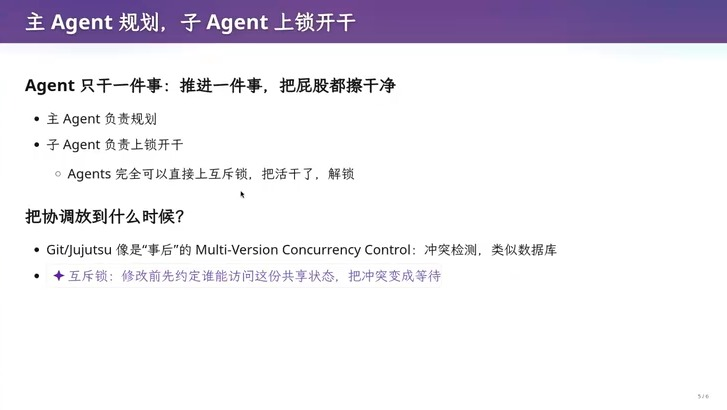
\includegraphics[width=\textwidth]{figures/fig_20_main_sub_agent_lock.jpg}
\caption{主 Agent 规划、子 Agent 上锁开干的协作模型，以及 Git/Jujutsu 作为“事后”式多版本并发控制的定位\vtag}
\end{figure}
\srcnote{00:55:30--00:55:44}

操作系统课里学的是悲观并发控制：访问可能冲突的资源前先 acquire 一把锁，别人要 lock 就必须等它 release，形成“先一后二”的次序；使用资源前必须声明（declare）对它的使用。讲者把这概括为“一把大锁保平安”。落到 Agent 协作，规则是：主 Agent 规划完立刻锁住要做的 scope，锁住后才动手，做完 commit，再解锁；目标已被别人锁住就等待。粒度可以选文件级锁，避免两个 agent 同写一个测试或配置文件。悲观并不必然低吞吐——只要系统里还有大量独立、不冲突的线程，即便各自持锁仍能高效推进；代价是锁把本来可并发的程序退回串行，与多处理器并行存在根本矛盾，细粒度锁只能缓解，无法取消。

\begin{lstlisting}[caption={幻灯片给出的 git worktree 用法：为每个 Agent 建一条分支和一个工作目录}]
git worktree add -b agent-a ../gense-agent-a
git worktree add -b agent-b ../gense-agent-b
\end{lstlisting}

\begin{table}[H]
\centering
\begin{tabular}{p{2.2cm}p{6.2cm}p{6.6cm}}
\toprule
 & 乐观并发控制（Git 一类） & 悲观并发控制（锁） \\
\midrule
核心假设 & 两个事务大概率不冲突 & 冲突随时可能发生 \\
协调时机 & 事前开会，事后检测 & 使用资源前先约定 \\
冲突的表现 & 合并时冲突、abort 回滚 & 冲突变成等待 \\
主要代价 & 大量并行时 abort 频繁 & 把可并发的部分退回串行 \\
\bottomrule
\end{tabular}
\caption{乐观并发控制与悲观并发控制的对照}
\end{table}

锁保护什么，幻灯片给的界定是“一件事依赖的共享状态”：只锁正在写的文件，可能漏掉别人正在改的接口；与数据库的 advisory lock 一样，所有参与访问的 agent 都要遵守协议，而锁不会自动让错误的修改变正确。完整协议是上锁、读取最新状态、修改、验证并留下可恢复快照、解锁。

\begin{warningbox}{锁保护的是“依赖的共享状态”}
锁的边界不在被修改的文件本身，而在“把活干完”所依赖的共享状态；协议靠参与者自愿遵守，锁只保证互斥，不保证正确。
\end{warningbox}

\begin{figure}[H]
\centering
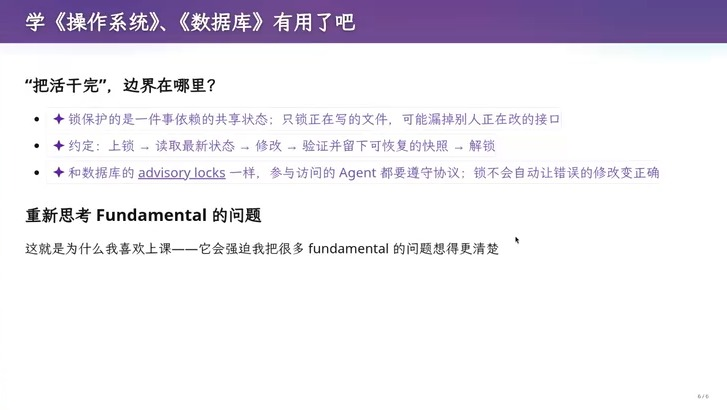
\includegraphics[width=\textwidth]{figures/fig_21_lock_boundary.jpg}
\caption{锁保护的是一件事所依赖的共享状态，以及“上锁、读取最新状态、修改、验证并留下快照、解锁”的完整协议\vtag}
\end{figure}
\srcnote{01:02:30--01:02:44}

\subsection{本章小结}

Git 可理解为“事后的、乐观的多版本并发控制”：先各自往前跑，合并时再检测冲突，假设由读写局部性支撑。Agent 提速、协调不克制时假设失效，讲者主张转向悲观控制：规划后锁住 scope，先声明再使用，冲突变成等待；锁粒度至少覆盖一件事依赖的共享状态，并且要靠所有参与者遵守协议。

\section{版本控制之后：团队复杂度与 AI 斩杀线}

版本管理讲完，讲者加了一句限定：它本质上还是一个工具，不管乐观还是悲观，真正困难的是进度即团队管理。他给出一个可检验的判据，称为“斩杀线”：如果老板随口一句“我要做一个 agent 用的微信”“做一个 AI 时代的微信”要它成为社交爆款，AI 就能直接产出那个微信级产品，软件工程就死了，“那我们就都死了”。他随即说这条线暂时还没到，至少没到团队管理这一层；但“我觉得可能也许有一天真的我也要被斩杀”——“我觉得”“可能”“也许”三重限定。

支撑判断的既有观察是缩放律：摩尔定律还成立，模型会更强、更小、更快，算力也许有一天能换出智能；但今天 AI 还不知道怎么做团队管理。

\begin{figure}[H]
\centering

\includegraphics[width=\textwidth]{figures/fig_22_team_kill_line.jpg}
\caption{版本控制只是工具，真正的困难在进度（团队）管理；AI 是一条斩杀线\vtag}
\end{figure}
\srcnote{01:03:45--01:03:59}

团队管理难在沟通关系平方级增长：每多一个人，沟通关系都平方级上升。幻灯片给出公式

\[ C(n) = \frac{n(n-1)}{2} \]

其中 $n$ 是人数，$n-1$ 是每人需要沟通的其他成员数，除以 2 是因为同一对关系只计一次；代入幻灯片例子，5 人对应 10 条，10 人对应 45 条。公式、数字与所引的 Brooks《人月神话》都出自幻灯片；讲者口播只说“人月神话里面，就是人之间两两之间是平方级的沟通关系”（转写记成“人乐神话”），没有念作者名与公式。

后果并不抽象：即便各人做好分内事，由于平方级沟通关系，你不完全知道别人在做什么，仍会冲突——“你写测试我过不了”经常发生。幻灯片把“我的部分已经好了”背后的失效归为四类：目标不一致（你要赶紧上线、我要趁机重构，两人都觉得自己在帮项目）、依赖在等待（前端等接口、后端等需求，关键路径没动）、完成的定义不同（我的代码能跑，你以为能交付，一集成才发现理解不同）、责任落在缝隙里（接口、测试、部署都有人负责，跨模块问题没人认领）。

\begin{figure}[H]
\centering

\includegraphics[width=\textwidth]{figures/fig_23_brooks_complexity.jpg}
\caption{人数增加带来平方级的潜在沟通关系：5 人 10 条，10 人 45 条\vtag}
\end{figure}
\srcnote{01:05:45--01:05:59}

稀缺的因此是能分解任务的人：最难招的是能把一个 100 人团队分出 10 个小团队、拼起来仍是一个团队的 team leader，其次是能带小团队的人。讲者给学生的练习是把自己当主 Agent，用两三个或更多 agent，想清楚任务如何分解、以及提交策略——何时提交、何时合并。

版本控制最终留下的是一种定位与一组 first principles：它是工具，凝结了人类过去很多年软件工程的经验，说的是“我们人类要这样开发”；在此之上才长出你自己的直觉与经验。幻灯片总结为“记住历史、并行探索、汇合成果”——项目可以不只是“当前状态”，要能看到历史、记住教训，也能管理多个并行探索并最终合并，失败尝试同样留下教训；技术会过时，first principles 会留下。讲者对“记住教训”留了口子：它也许会被 Agent Memory 替代。

\begin{figure}[H]
\centering
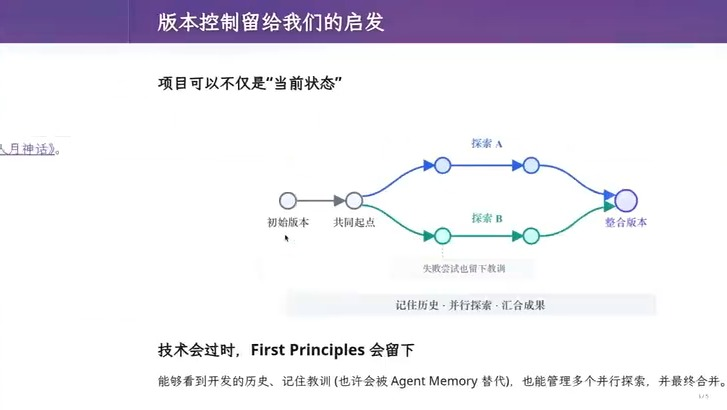
\includegraphics[width=\textwidth]{figures/fig_24_vcs_lessons.jpg}
\caption{版本控制留下的启发：项目不只是当前状态，失败的探索也留下教训\vtag}
\end{figure}
\srcnote{01:06:45--01:06:59}

\begin{importantbox}{本节的判断边界}
“版本控制是工具”“真正的困难是团队管理”是讲者的明确判断；“AI 是一条斩杀线”是他提出的判据，并明确说线暂时还没到；“我也要被斩杀”带三重弱化词。三者不应写成同一确定度。
\end{importantbox}

\subsection{本章小结}

版本控制收束为一件工具，真正难题在进度与团队管理，其量级由 n(n-1)/2 的沟通关系决定，因此最能分解任务的人最稀缺。讲者给学生的落点是把自己当主 Agent 练习任务分解与提交策略；留下的 first principles 是记住历史、并行探索、汇合成果。

\section{从产品需求到 Git：记录做题轨迹为什么不需要数据库}

Pico Playground 是讲者讨论"需求决定工具"的具体产品：给小学生做汉诺塔题，额外限制是所有盘子只能朝一个方向移动。约束改变了递归结构，最大盘每步右移一格，小盘子问题由归纳法保证最优。产品要卖的不是答案而是过程：只保存最终盘面看不出孩子卡在哪里，只有把动作存成逐行文本，才能回放、比较、点评。

增值服务是免费 playground 加付费 AI 助教：孩子做不下去时点"我要助教"，模型给出个性化指导；收费按高于 DeepSeek 原价的 token 费计到用户账户，prompt 是"有经验的老教师"经验的蒸馏。它引出的技术问题是做题记录要在服务器端保存。

\begin{figure}[H]
\centering
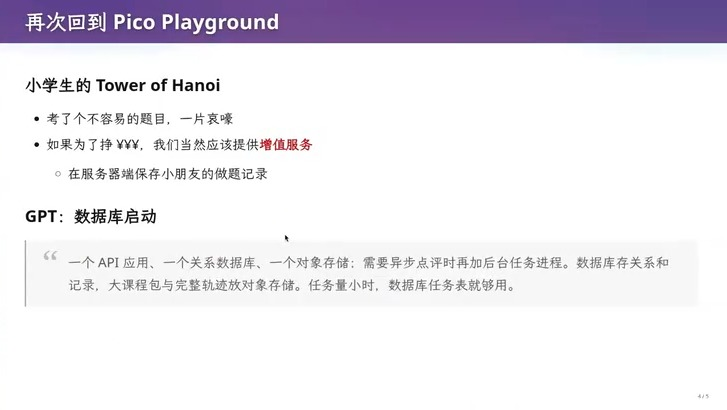
\includegraphics[width=\textwidth]{figures/fig_25_pico_tower_hanoi.jpg}
\caption{回到 Pico Playground：小学生的 Tower of Hanoi 与"数据库启动"的设想\vtag}
\end{figure}
\srcnote{01:08:15--01:08:29}

GPT 给出的方案是"一个 API 应用、一个关系数据库、一个对象存储，需要异步点评时再加后台任务进程；数据库存关系和记录，大课程包与完整轨迹放对象存储，任务量小时数据库任务表就够用"。讲者说"我不喜欢这个设计"，理由不在技术对错，而在需求错位：他真正要的是版本管理。

Git 恰好提供了版本管理需要的东西：树状版本历史留下"做到哪一步、从哪里重试"；两次提交之间的免费 diff 回答"到底改了什么"；Comment Commit 与 git notes 把点评关联到当时版本，可以后补而不改原提交。交互设想是学生每改一次、空闲、点运行或切换界面时自动提交一次 Git，申请 AI 助教时就在这次提交上长出分叉，把点评挂上去。

\begin{knowledgebox}{Git 为轨迹记录提供的三样现成能力}
树状版本历史保留"做到哪一步、可以从哪里重试"；提交之间的 diff 免费给出前后变化；git notes 把点评绑定到当时的版本，事后可补写而不重写原提交；"哪一步值得表扬"仍由应用层理解。
\end{knowledgebox}

\begin{table}[H]
\centering
\begin{tabular}{p{1.6cm}p{6.4cm}p{6.4cm}}
\toprule
维度 & 关系数据库方案 & Git 记录方案 \\
\midrule
记录对象 & 关系与记录、大对象另存 & 动作序列的逐行文本（快照） \\
历史与重试 & 需要自行设计 & 树状版本历史，做到哪一步可留下 \\
差异查看 & 需要自行实现 & 免费 diff，直接看两次提交改了什么 \\
点评关联 & 需要另建关联表 & Comment Commit 与 git notes，可后补 \\
早期迁移成本 & 每次 schema 改动都要迁移 & 目录与提交信息格式可先探索后收敛 \\
\bottomrule
\end{tabular}
\caption{记录做题轨迹时，数据库方案与 Git 方案的取向对比}
\end{table}

幻灯片里的汉诺塔实现只有 next\_of 与 hanoi 两个短函数。幻灯片 OCR 有字符被识别成小写 c 或断行，以下片段按幻灯片呈现节选。

\begin{lstlisting}[caption={幻灯片中的汉诺塔最小实现（节选，OCR 还原）}]
def next_of(peg):
    return {"A": "B", "B": "c", "c": "A"}[peg]

def hanoi(n, src, dst):
    aux = set("ABc") - (src, dst)
    ...
\end{lstlisting}

\begin{figure}[H]
\centering
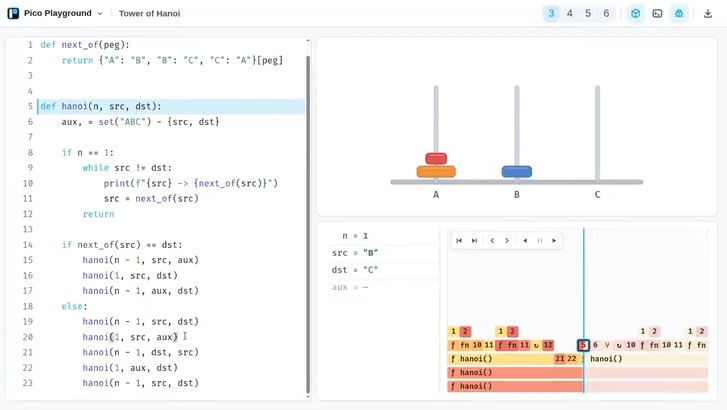
\includegraphics[width=\textwidth]{figures/fig_26_hanoi_code.jpg}
\caption{幻灯片给出的 Tower of Hanoi 最小实现：next\_of 与 hanoi\vtag}
\end{figure}
\srcnote{01:11:45--01:11:59}

讲者的成本判断是：产生一次 Git 提交的成本远远小于把其余状态持久化下来的成本，可以忽略；数据库能换来更小的压缩体积和更高的性能，但那不是需求。早期策略是先把代码放进自己的代码库，用 Git 探索，直到文件目录格式、commit message 格式与使用方式都收敛，再迁移到数据库。

\begin{figure}[H]
\centering
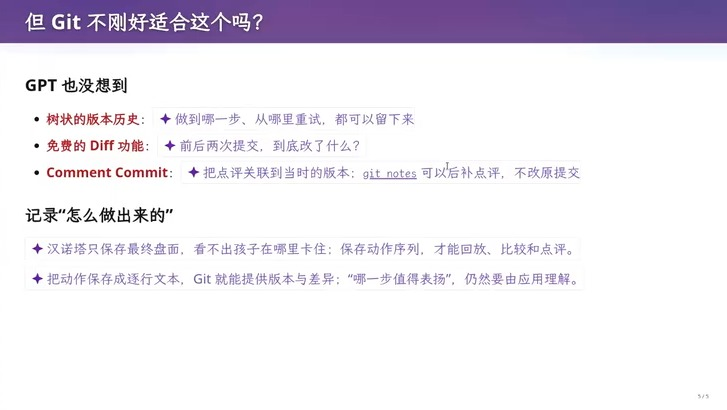
\includegraphics[width=\textwidth]{figures/fig_27_git_fits.jpg}
\caption{但 Git 不刚好适合这个吗：树状历史、免费的 diff 与 git notes\vtag}
\end{figure}
\srcnote{01:15:00--01:15:14}

版本管理只是工具，也决定从零开始时人的角色：早期不用 Multi-Agent，"你就是包工头"，先找你能用到的最强 Agent 多轮对话；Multi-Agent 更适合已经成形的项目。"任何时候，开始都比不开始强"，讲者当场打开课程作业开始写。

\begin{figure}[H]
\centering
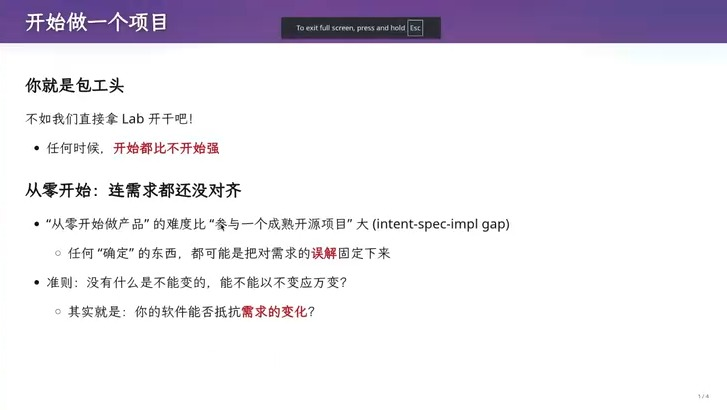
\includegraphics[width=\textwidth]{figures/fig_28_start_project.jpg}
\caption{开始做一个项目：你就是包工头，从零开始连需求都还没对齐\vtag}
\end{figure}
\srcnote{01:18:00--01:18:14}

\subsection{本章小结}

要保存的是动作序列而不是最终盘面；"API 应用 + 关系数据库 + 对象存储"被讲者因需求是版本管理而否决。树状历史、免费 diff 与 git notes 覆盖记录、比较、点评，一次提交的成本远低于持久化其余状态，所以早期用可读可改的文件与仓库承载，格式收敛后再迁移数据库。

\section{提示词工程与从零构建：intent--spec gap 与过度遵循}

现场演示从 \texttt{/tmp/lab1} 开始，讲者用 pi（0.85.1）配合 deepseek-v4-flash 起了一个空目录。一线模型面对开放需求会进入 plan mode、确认事实、生成 workflow；Claude Code 这类工具在复杂任务里会生成 JavaScript 或 TypeScript，其中有个名为 agent 的函数，函数体是自然语言，甚至用循环组织多个任务。讲者形容生成速度为"这个 300 token per second，实在是太恐怖了"。

危险点在提示词工程的机制：提示词里的每一句、每一个词 self-attention 都会看到；模型已被训练成遵循指令，带着"没有办法往外拉的倾向"，面对讨论稿不会保留模糊性，反而过度遵循字面指令，生成"确实满足了指令，但是其实不是你想要的"东西。

实验要求列了很多条，真正重要的是"实现一个持续为你工作的个人助手"，其余都只是解读。讲者想要的第一个 feature 是学习——高校学习与复习、要"捡成绩"；他要能自动从外网收集数据、层次化归档、再给一个好用的界面。现场 agent 没沿这条线走，它在做 database。

\begin{importantbox}{过度遵循指令为什么危险}
指令进入上下文后没有"轻重"之分，self-attention 会平等地看到每一句话；模型被训练成尽量服从，会把讨论稿当成定稿、把字面要求当成目标。结果是每一条要求都不算错，整体却偏离真实意图。风险的本体是：需求文档的主句被淹没了。
\end{importantbox}

讲者把这叫 intent 与 specification 之间的巨大 gap：agent 看到"要实现这个"就真的去实现；没有精心设想、讨论过的时候，AI 基本上只会生成 slop，看起来每件事都对、没有错误，最终却得到你不想要的东西。边界是：一号（ehall）只是测试出口和个人信息入口，真正需要的是 browser use agent，第一步不必在教育系统上做太多设计。

现场还暴露 agent 甚至没有创建 git repository。管理要先于编码：成熟产品经理在写下第一行代码前会先和团队谈协作、项目管理和每天何时开会。准则是先创建一个空仓库，再想下一步迈向哪里，且只能往前迈一小步。讲者判断，AI 从零做 slop 的难度比在成熟项目里做维护性任务大很多。

版本管理收敛成三件事：记住现在、记住历史、记住教训。记住现在，是因为要有 repository 把文件管起来（C、C++、Python、JS 都一样）；记住历史，是因为删掉的东西可能有用还能捞回；提交历史让你看到如何演进、某条路失败后回到另一个点走正确路线。这些 lessons 保存在版本控制里，在 agent 时代和"古法编程"时代都成立。

讲者用"你能不能以不变应万变"收束：现在设计的架构、流程方法能否抵抗未来需求发生根本性的变化？AI 助教可能是文字的、图像的、有交互的、无交互的，架构要用最少变化应对。这是软件工程与数据库、操作系统课程最不同的地方。

\begin{figure}[H]
\centering
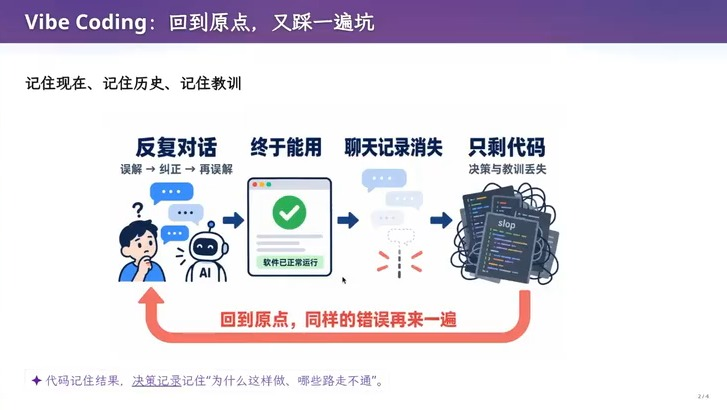
\includegraphics[width=\textwidth]{figures/fig_29_vibecoding_lessons.jpg}
\caption{Vibe Coding 的教训：代码记住结果，决策记录记住"为什么"与"哪些路走不通"\vtag}
\end{figure}
\srcnote{01:29:30--01:29:44}

\begin{lstlisting}[caption={现场演示中真实出现的命令与输出（逐字保留）}]
$ eza --git --group-directories-first --icons=auto
$ cd pico-playground/
$ npm run dv
npm error Missing script: "dv"
$ npm run dev
> learn-python@1.0.0 dev
> node scripts/dev.mjs
...
dev server: http://localhost:5173/
$ chr
fish: Unknown command: chr
$ git status
fatal: not a git repository (or any parent up to mount point /)
Stopping at filesystem boundary (GIT_DISCOVERY_ACROSS_FILESYSTEM not set).
\end{lstlisting}

\subsection{本章小结}

提示词承担规格说明的角色，却带有被过度遵循的风险：每句话都被 self-attention 看到，模型服从字面要求，intent 与 specification 出现巨大 gap。这份实验要求真正的主句只有"实现一个持续为你工作的个人助手"；agent 默认不建仓库，版本管理要靠人立规矩。

\section{MVP 与架构弹性：先文件系统，再数据库，以及云盘同步的硬红线}

评审 agent 的产出时，它做了一个提交，手机端是真实 HTTP 服务，ehall 与邮件用 fixture 模拟；分层为入口层（pi 扩展、CLI、手机 PWA、daemon）、编排层（workflow、executor、brain、archive）、能力层（smail、pdb、ehall）、核心层（配置、确认状态机、数据库 schema、任务队列、审计）、数据层（\texttt{data/pdb} 真源、\texttt{state/assistant.db} 单库、\texttt{data/fixtures}）。分层没问题，问题是它被当成业务逻辑系统来做，看起来已像教务系统，把尚未确认的需求固化成了抽象。

\begin{figure}[H]
\centering
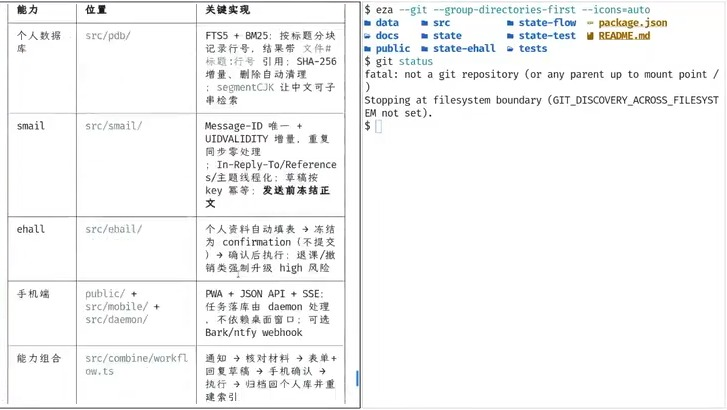
\includegraphics[width=\textwidth]{figures/fig_30_capability_table.jpg}
\caption{能力、位置与关键实现：个人数据用 FTS5+BM25 分块索引并保留行号引用\vtag}
\end{figure}
\srcnote{01:30:45--01:30:59}

这套设计把"危险动作不能自动发生"写成规则：个人数据只存 Markdown，索引用 FTS5+BM25 按标题分块，结果带"文件与标题、行号"引用，按内容哈希增量、删除自动清理；邮件用 Message-ID 唯一约束加 UIDVALIDITY 增量，重复同步零处理，草稿带 idempotency\_key；ehall 表单先冻结成 confirmation；所有对外动作穿过唯一闸门 executeConfirmation，状态机 pending 到 approved 到 executed 单向，markExecuted 带 WHERE status='approved'，对并发与重试幂等；确认时把主题、收件人、正文或表单字段写进 payload，执行时读 payload 而非草稿；风险按服务元数据分 Low、medium、high，标题命中退课、撤销、注销自动升 high，medium 输"确认"，high 输"我确认执行"；手机任务落 tasks 表，由 daemon 原子领取，关掉手机照跑。

\begin{figure}[H]
\centering
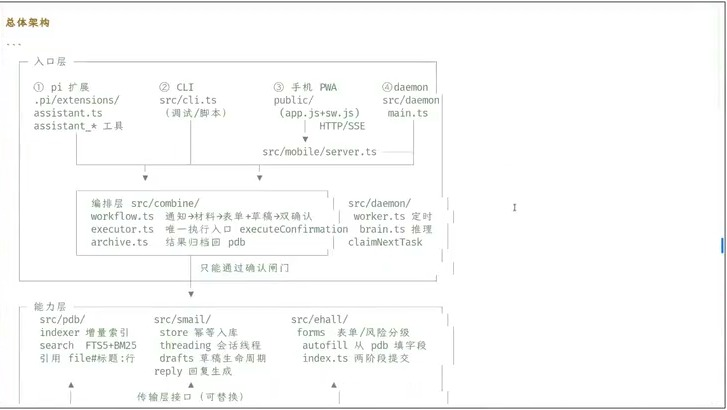
\includegraphics[width=\textwidth]{figures/fig_31_architecture.jpg}
\caption{总体架构：pi 扩展、CLI、手机 PWA 三个入口，daemon 与分层能力\vtag}
\end{figure}
\srcnote{01:32:00--01:32:14}

自测让仍在 pending 的 confirmation 直接执行，被拒绝：必须先批准，未执行任何操作。外部连通性验证得到 \texttt{imap.smail.nju.edu.cn:993} TCP 可连，统一身份认证登录页返回 HTTP 200、27855 bytes，能解析出 execution token。诚实边界是：demo 用 fixture 保证可复现、不碰真实数据；核心逻辑、HTTP 服务和 pi 工具调用是真执行；live 适配器只验证到 TCP 连通与 CAS 页面可解析 token，真实登录与提交因无凭据未闭环。

讲者认为更符合 best practice 的是 MVP：Minimum Viable Product，给一个立即能用、不完备的版本，帮你考虑未来变化、评估设计。他引"the biggest risk in product development, is building something nobody wants."，并口误说成 minimum variable product；幻灯片署名 Eric Ries。

\begin{figure}[H]
\centering
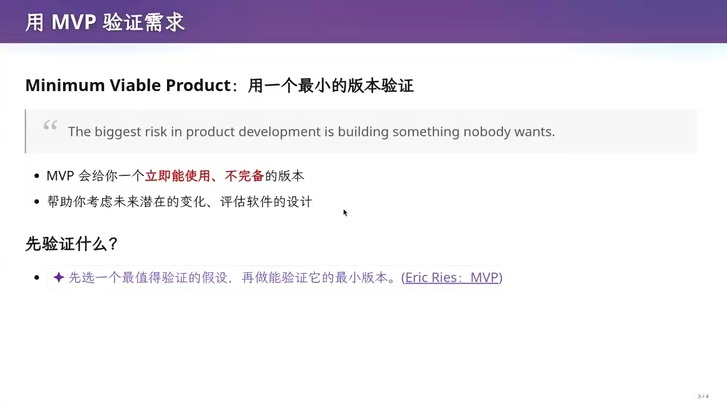
\includegraphics[width=\textwidth]{figures/fig_32_mvp.jpg}
\caption{用 MVP 验证需求：先选一个最值得验证的假设，再做能验证它的最小版本\vtag}
\end{figure}
\srcnote{01:32:30--01:32:44}

\begin{knowledgebox}{MVP 的用法}
MVP 不是"先做简化版再加功能"，而是先选一个最值得验证的假设，只做能验证它的最小版本。讲者据此要求先回答"什么样的需求才是绝对要的"：对他自己而言是提升学习效率的能力和提升工作效率的能力。
\end{knowledgebox}

第一处选型改变是第一个 MVP 可以没有任何数据库。带数据库后每次重构都要让 agent 做 database migration，文件系统则可以自己调整目录结构；调文件与调 database schema 的心智负担也不同，人从小熟悉文件目录，不熟悉的 schema 要先做概念翻译。讲者自己的回邮件 agent 就不用数据库：收邮箱，把 email ID 放到共享云盘同步，email ID 带回复草稿和邮件分类（是否垃圾邮件），再由下一级流水线处理；关键是想清有哪几级流水线、如何协作、哪些通过云盘传递。

\begin{figure}[H]
\centering
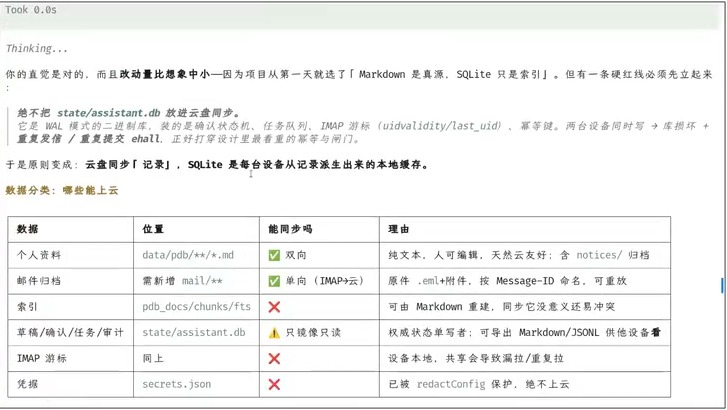
\includegraphics[width=\textwidth]{figures/fig_33_cloud_sync_redline.jpg}
\caption{硬红线：绝不把 state/assistant.db 放进云盘同步\vtag}
\end{figure}
\srcnote{01:36:30--01:36:44}

需求变更出现：希望邮件资料等与云盘同步。它检验架构——现在也许满足需求，需求变化时的改动是摧毁性的、背上技术债还是别的，"那就不知道了"。当前把个人资料、邮件归档、索引、草稿都放在一个 \texttt{state/assistant.db}，短期不会有大问题；往后分两条路：一上来做大系统、几步实现完、拖技术债迭代，或从最小处得到精巧架构。讲者举例：用 Git 管理学生提交后，很多事变容易、自己也更好控制，所以在遇到性能瓶颈前不打算迁移到任何数据库。

云盘方案第一条是硬红线：绝不把 \texttt{state/assistant.db} 放进云盘同步。它是 WAL 模式的二进制库，装着确认状态机、任务队列、IMAP 游标（uidvalidity 与 last\_uid）和幂等键；两台设备同时写会库损坏，甚至重复发信、重复提交 ehall。原则是云盘同步"记录"，SQLite 是每台设备从记录派生的本地缓存。

\begin{warningbox}{云盘同步的硬红线}
数据库文件不能进云盘，因为它不是普通文件，而是带 WAL 日志的二进制库，其中保存着决定外部动作是否重复的游标与幂等键。两台设备并发写会破坏一致性，并可能把"确认一次、执行一次"的保证变成重复提交。可同步的是记录本身；SQLite 只作为本地的派生物。
\end{warningbox}

\begin{table}[H]
\centering
\begin{tabular}{p{1.7cm}p{3.8cm}p{2.1cm}p{6.9cm}}
\toprule
数据 & 位置 & 能否同步 & 理由 \\
\midrule
个人资料 & \texttt{data/pdb} 下的 Markdown & 双向 & 纯文本，人可编辑，天然云友好 \\
邮件归档 & 需新增 mail 目录 & 单向（IMAP 到云） & 原件与附件，按 Message-ID 命名，可重放 \\
索引 & pdb 文档与分块、FTS & 不同步 & 可由 Markdown 重建，同步无意义且易冲突 \\
状态库 & \texttt{state/assistant.db} & 只镜像只读 & 权威状态单写者，可导出供他设备查看 \\
IMAP 游标 & 设备本地 & 不同步 & 共享会导致漏拉或重复拉 \\
凭据 & \texttt{secrets.json} & 绝不上云 & 已被 redactConfig 保护 \\
\bottomrule
\end{tabular}
\caption{哪些数据可以上云：按数据类别决定同步方向与权威位置}
\end{table}

六项改动：配置加 cloud 段（enabled、transport、root、remoteDir 等，pdbDir 允许指向云盘挂载点）；新增 \texttt{cloud\_state} 表存同步游标（path、hash、etag、mtime、dir、updated\_at，存本地）；archive 从追加 \texttt{notices/YYYY-MM.md} 改成一事一文件 \texttt{notices/2025-09/确认 ID.md}，用确认 ID 命名得到确定性、幂等并避免冲突；新增 \texttt{cloud/exporter} 把邮件写成 .eml 与附件；daemon tick 里做 cloud.sync，新文件则 reindex 并用 SSE 通知手机；多设备写权限用单写者租约（\texttt{locks/daemon.lock} 加心跳）或按设备分片、读全部只写自己。落地三档与冲突处理见下表。推进顺序是先只改 pdbDir 加 watcher 当天可用，再抽 \texttt{src/cloud} 并把 archive 改成一事一文件，最后加 mail exporter；先立"SQLite 不出本机"和"一事一文件"两条规矩，否则云盘会让幂等设计从内部崩掉。

\begin{table}[H]
\centering
\begin{tabular}{p{2.3cm}p{6.0cm}p{6.0cm}}
\toprule
方案 & 改动 & 冲突处理 \\
\midrule
A 挂载目录 & 几乎零代码，加 \texttt{fs.watch} 触发 reindex & 云客户端生成冲突副本，够用 \\
B WebDAV 适配器 & 新增 \texttt{src/cloud} 一层 & etag 可信，可做精确三方比对（推荐） \\
C 网盘 API & OAuth 加分片上传 & 无稳定 etag，冲突检测难，只适合单向备份 \\
\bottomrule
\end{tabular}
\caption{引入云盘的三种落地方式及其冲突处理能力}
\end{table}

\begin{figure}[H]
\centering
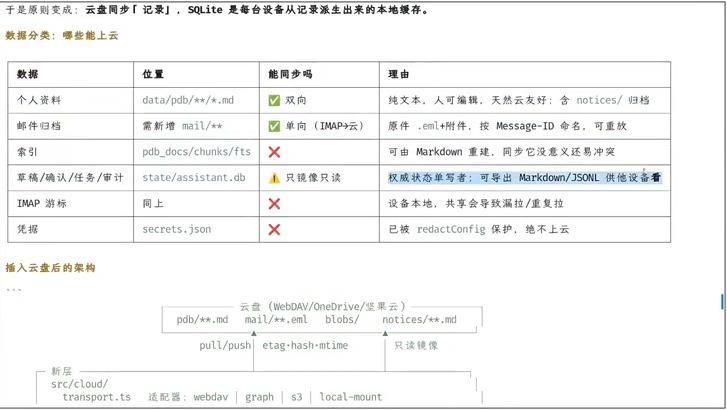
\includegraphics[width=\textwidth]{figures/fig_34_data_classification.jpg}
\caption{数据分类：哪些能上云，哪些只能由本机从记录派生\vtag}
\end{figure}
\srcnote{01:37:00--01:37:14}

最后的落点是 prompt 的杠杆效应：早期 prompt 对整个项目的走向影响最大，任何被"确定"下来的设计都会变成潜在的 technical debt。留下历史、让自动提交与 push 形成可留痕的历史，可用的版本还能帮助你重新整理架构设计。

\begin{figure}[H]
\centering
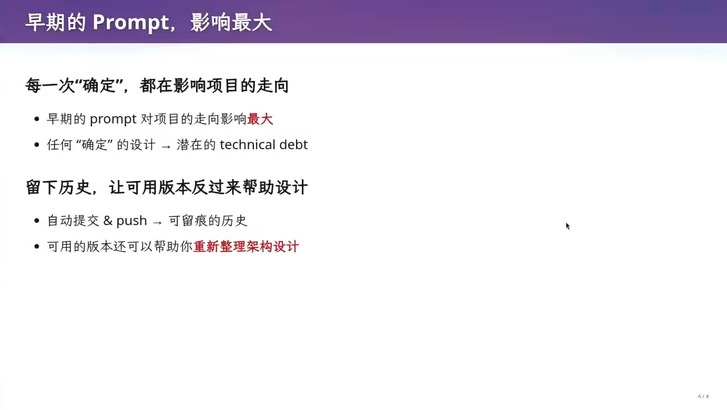
\includegraphics[width=\textwidth]{figures/fig_35_prompt_tech_debt.jpg}
\caption{早期的 prompt 影响最大：每一次"确定"都在埋下技术债\vtag}
\end{figure}
\srcnote{01:38:00--01:38:14}

\subsection{本章小结}

讲者的批评不在分层，而在把未确认的需求过早固化成业务系统。更符合 best practice 的是先做 MVP：选一个最值得验证的假设，只做能验证它的最小版本；第一个 MVP 可以没有数据库。需求变成"与云盘同步"后，第一条是硬红线：数据库文件不进云盘，云盘同步记录，SQLite 只做本机派生缓存。早期 prompt 影响最大，每次"确定"都可能成为技术债，要留下可回退的历史。

\section{总结与延伸}

这一讲的主线可以压成一句话：版本管理系统的形状，由它假定的使用者决定；当使用者从人变成并行工作的 Agent，原先合理的假设就开始失效。讲者没有给出一个「标准答案」，而是把 Git 与 Jujutsu 的设计摆在一起，让读者自己看清每一步取舍的理由。

\subsection{讲者给出的收束}

讲者的落点不在某个具体工具。他在结尾反复强调，课程教的不是 Git 操作，而是生成式软件工程：版本控制凝结了人类过去在协作中吃过的亏——需要历史、需要并行探索、需要把成果汇合起来，也需要知道「为什么这样做、哪些路走不通」。这些需求不会因为模型变强而消失，只是执行它们的主体从人换成了 Agent。他同时提醒，团队管理与进度管理才是真正的难点，版本控制只是工具；所谓 AI 的「斩杀线」暂时还没有到来，但「也许有一天」会轮到讲者自己。课程在「下一次会讲软件架构与构造」的交接中结束，本讲的内容构成后续讨论的地基。

\subsection{本讲义的结构化提炼}

把全讲压缩成一条因果链，可以这样复述：

\begin{importantbox}{一句话机制链}
现有版本管理工具默认使用者是人：单线程、change 以小时计、沟通比提交慢，因此用快照和分支来组织历史是合理的。Agent 把这些前提同时改掉——原子提交降到秒级、多个写者并行、克隆体不怕追责——于是「用 commit 代表 change」的代理结构开始别扭。Jujutsu 把 change 提升为一等公民来修复身份问题；\texttt{git worktree} 用共享对象库加多个工作目录来容纳并行；锁把并发从执行推回协调。最后仍然要回到人的问题：谁规划、谁在什么粒度上确认、教训存在哪里。
\end{importantbox}

四个机制值得单独记住。第一，change 与 commit 是两种身份：commit ID 描述一次快照，change ID 描述一次修改意图，重写历史时前者会变、后者应当延续。第二，工作副本本身可以是 commit，这消掉了 staging area 这一层，也解释了为什么冲突可以直接存进 commit 而不必中断历史。第三，\texttt{git worktree} 让一个仓库拥有多个工作目录，各自持有 HEAD 与 index，却共享对象库与分支引用，因此本地并行不需要远程往返。第四，并发控制没有免费选项：乐观方案假设冲突稀少并靠事后合并修复，悲观方案用锁把冲突挡在门外，代价是把并行退回串行，而且锁只能保护参与者约定保护的那部分共享状态。

\subsection{可以直接使用的判断}

\begin{itemize}
  \item 并行 Agent 写同一个仓库时，先判断冲突是否真的稀少。访问局部性强，乐观方案便宜；多个 Agent 频繁碰同一测试或配置文件，就该把粒度缩到可锁的共享状态。
  \item 用锁保护的不只是「正在写的文件」。一个任务依赖的接口、配置、测试都算共享状态，只锁文件会让别人改到接口却无人察觉。
  \item 锁协议要和数据库的 advisory lock 一样被所有参与者遵守：上锁、读取最新状态、修改、验证并留下可恢复的快照、解锁。锁本身不会让错误的修改变正确。
  \item 记录「为什么」和记录「改了什么」同样重要。代码记住结果，决策记录记住当时为什么这样选、哪些路走不通；后者在需求变化时才是可复用的资产。
  \item 项目早期的 prompt 影响最大。每一次「确定」都会把某种理解固定下来，也就埋下技术债，因此能回退、能重做，比一次做对更现实。
\end{itemize}

\subsection{边界与开放问题}

本讲有几个明确的未决点，读者不宜把它们当成结论。第一，模型能否「一步生成」大型项目，讲者自己说「我们现在还不知道」。第二，让 AI 在内部维护 artifact 一致性、生成可视化视图、甚至让人不再阅读代码，讲者用「未来有可能发生的」来限定，属于预测而非已验证事实。第三，Agent 快一千倍时乐观并发控制会更频繁地 abort，讲者认为这在 AI 时代「也不是什么大问题」，理由是 Agent 能够自我修复，这一判断依赖模型能力继续提升。第四，团队复杂度按 n(n-1)/2 增长、以及在多大程度上能由 Agent 替代沟通，本讲只给出方向与直觉。

真正值得继续追问的是：当写代码的边际成本趋近于零，我们要优化的是提交速率、验证速率，还是「值得被记住的决策」的密度？这也正是下一讲软件架构与构造要接着回答的问题。
%% --- 正文内容结束 --- %%

\end{document}
